\documentclass[11pt,a4paper]{article}
\usepackage{fix-cm}
\usepackage{amsmath,amssymb,amsfonts,graphicx,bm}
\usepackage{xr-hyper}
\usepackage{hyperref}
\usepackage[hypcap=false]{caption}
\usepackage{placeins,microtype,xurl,float}
\usepackage[margin=1in]{geometry}
\usepackage[backend=biber,style=numeric,sorting=none]{biblatex}
\addbibresource{supplement-references.bib}
\externaldocument[M-]{fwm-and-coupler}
\renewcommand{\thesection}{S\arabic{section}}
\renewcommand{\theequation}{S\arabic{equation}}
\renewcommand{\thefigure}{S\arabic{figure}}
\renewcommand{\thetable}{S\arabic{table}}
\renewcommand{\thepage}{S\arabic{page}}
\begin{document}
\title{Supplement 1: Elliptic complex-envelope solutions and normal forms for four-wave mixing and coherent couplers}
\author{Graham Hesketh \\
\small Independent researcher, United Kingdom}
\date{\today}
\maketitle
This supplement retains the detailed derivations, chart data, reconstruction formulas and numerical inputs supporting the main paper.
Mathematical notation is unchanged; its scope follows the indicated FWM, coherent-coupler and lifted systems.
Section, equation, figure and table numbers prefixed by S belong to this supplement; other numbered cross-references refer to the main paper.
The central method and results are presented in the main paper; this supplement provides their detailed verification and evaluation.

\section{Physical FWM normalisation}\label{supp:sec:physical}
In this section we recall the four-wave mixing system from nonlinear fibre optics that forms the focus of our study.
The coupled system of ordinary differential equations in \eqref{eq:fwm-system} is taken from \cite{agrawalNonlinearFiberOptics2019} which references \cite{stolenParametricAmplificationFrequency1982} as the origin of the theory.
The system describes four-wave mixing in the quasi-continuous-wave limit, i.e., when temporal envelope variations are negligible compared to the spatial evolution along the propagation direction, allowing time derivatives to be neglected.
Physically, the equations describe the evolution of four copropagating optical waves that exchange energy through the Kerr nonlinearity.
Each wave experiences self-phase modulation (SPM), where its own intensity induces a phase shift on itself, cross-phase modulation (XPM), where the intensities of other waves induce additional phase shifts, and parametric coupling through the four-wave mixing terms, which enable direct energy transfer between the waves when phase-matching conditions are satisfied:
\begin{align}
\frac{dA_1}{dz} &= \frac{in_2\omega_1}{c}\left[\left(f_{1,1}|A_1|^2 + 2\sum_{k\neq 1} f_{1,k}|A_k|^2\right)A_1 + 2f_{1,2,3,4}A_2^*A_3A_4e^{i\Delta kz}\right], \notag \\
\frac{dA_2}{dz} &= \frac{in_2\omega_2}{c}\left[\left(f_{2,2}|A_2|^2 + 2\sum_{k\neq 2} f_{2,k}|A_k|^2\right)A_2 + 2f_{2,1,3,4}A_1^*A_3A_4e^{i\Delta kz}\right], \notag \\
\frac{dA_3}{dz} &= \frac{in_2\omega_3}{c}\left[\left(f_{3,3}|A_3|^2 + 2\sum_{k\neq 3} f_{3,k}|A_k|^2\right)A_3 + 2f_{3,4,1,2}A_1A_2A_4^*e^{-i\Delta kz}\right], \notag \\
\frac{dA_4}{dz} &= \frac{in_2\omega_4}{c}\left[\left(f_{4,4}|A_4|^2 + 2\sum_{k\neq 4} f_{4,k}|A_k|^2\right)A_4 + 2f_{4,3,1,2}A_1A_2A_3^*e^{-i\Delta kz}\right], \label{eq:fwm-system}
\end{align}
where:
\begin{itemize}
    \item $A_j$ are the slowly-varying complex field amplitudes for waves $j = 1, 2, 3, 4$
    \item $z$ is the propagation distance
    \item $\omega_j$ are the angular frequencies of the respective waves
    \item $c$ is the speed of light in vacuum
    \item $n_2$ is the nonlinear refractive index
    \item $f_{j,j}$ are the self-phase modulation (SPM) coefficients
    \item $f_{j,k}$ (for $j \neq k$) are the cross-phase modulation (XPM) coefficients
    \item $f_{j,k,l,m}$ are the four-wave mixing (FWM) coefficients
    \item $A^*$ denotes complex conjugation
    \item $\Delta k = -\beta_1 - \beta_2 + \beta_3 + \beta_4$ is the phase mismatch
    \item $\beta_j = n(\omega_j)\omega_j/c$ are the propagation constants.
\end{itemize}
The modal overlap integrals are defined in terms of the transverse distribution of the fibre mode $F_j(x,y)$ as:
\begin{align}
\label{eq:overlaps}
f_{j,k,l,m} &= \frac{\langle F_j^* F_k^* F_l F_m \rangle}{\sqrt{\langle |F_j|^2 \rangle \langle |F_k|^2 \rangle \langle |F_l|^2 \rangle \langle |F_m|^2 \rangle}}, \\
f_{j,k} &= f_{k,j} = f_{j,j,k,k}
\end{align}
where $\langle \cdots \rangle = \iint_{-\infty}^{\infty} (\cdots) \, dx\,dy$ denotes the transverse spatial integral. Agrawal says of \eqref{eq:fwm-system} that the equations ``are quite general in the sense that they include the effects of SPM, XPM, and pump depletion on the FWM process'' and stresses that numerical or approximate solutions are commonly utilised.
Herein, they are solved analytically.


% ---------- SECTION -------------
% --------------------------------

\subsection{Complex-envelope normalisation}
In this section we normalise and generalise the system, transforming it into a form that both simplifies the algebra and broadens the scope of applicability.
From \eqref{eq:overlaps}, we observe the following symmetries among the wave mixing coefficients:

\begin{align}
f_{1,2,3,4} &= |f_{1,2,3,4}|e^{i\varphi}, \notag \\
f_{2,1,3,4} &= f_{1,2,3,4} = |f_{1,2,3,4}|e^{i\varphi}, \notag \\
f_{3,4,1,2} &= f_{1,2,3,4}^* = |f_{1,2,3,4}|e^{-i\varphi}, \notag \\
f_{4,3,1,2} &= f_{1,2,3,4}^* = |f_{1,2,3,4}|e^{-i\varphi}, \label{eq:overlap-symms}
\end{align}
where $\varphi$ is the phase of $f_{1,2,3,4}$.
The symmetries in \eqref{eq:overlap-symms} follow directly from permutation of the first index pair and conjugation in \eqref{eq:overlaps}.
The scalar overlap formula itself is the modelling assumption; vectorial polarisation effects require the corresponding vector overlap model.
Assuming \eqref{eq:overlap-symms}, we can conveniently renormalise the functions, and also absorb the phase $\varphi$ as a global phase rotation of the modes in such a way that the wave mixing coefficients all become equal to one.

To do so, we introduce the following redefinition of physical complex envelopes $A_j, A^*_j$ in terms of abstracted variables $u_j,v_j$.
The complex conjugates $A, A^*$ are distributed among $u,v$ in a particular pattern (note that $u_3, u_4$ involve $A^*_3, A^*_4$ while $v_3, v_4$ involve $A_3, A_4$) so as to later give one product over $u$ and one over $v$ in the wave mixing terms:

\begin{align}
T &= \sqrt{\frac{2\,n_2 \left|f_{1,2,3,4}\right|}{c} \sqrt{ \prod\limits_{k=1}^{4} \omega_k}}, \label{eq:T-def} \\
u_1\left(z\right) &= \frac{T\,\,e^{-i\pi/4}\,e^{-i\varphi/4}}{\sqrt{\omega_{1}}} \,A_{1}\left(z\right)\,e^{i z \beta_{1}}, \notag \\
u_2\left(z\right) &= \frac{T\,e^{-i\pi/4}\,e^{-i\varphi/4}}{\sqrt{\omega_{2}}}\,A_{2}\left(z\right)\,e^{i z \beta_{2}}, \notag \\
u_3\left(z\right) &= \frac{T\,e^{i\pi/4}\,e^{-i\varphi/4}}{\sqrt{\omega_{3}}}\,A^*_{3}\left(z\right)\,e^{-i z \beta_{3}}, \notag \\
u_4\left(z\right) &= \frac{T\,e^{i\pi/4}\,e^{-i\varphi/4}}{\sqrt{\omega_{4}}}\,A^*_{4}\left(z\right)\,e^{-i z \beta_{4}}, \notag \\
v_1\left(z\right) &= \frac{T\,e^{-i\pi/4}\,e^{i\varphi/4}}{\sqrt{\omega_{1}}}\,A^*_{1}\left(z\right)\,e^{-i z \beta_{1}}, \notag \\
v_2\left(z\right) &= \frac{T\,e^{-i\pi/4}\,e^{i\varphi/4}}{\sqrt{\omega_{2}}}\,A^*_{2}\left(z\right)\,e^{-i z \beta_{2}}, \notag \\
v_3\left(z\right) &= \frac{T\,e^{i\pi/4}\,e^{i\varphi/4}}{\sqrt{\omega_{3}}}\,A_{3}\left(z\right)\,e^{i z \beta_{3}}, \notag \\
v_4\left(z\right) &= \frac{T\,e^{i\pi/4}\,e^{i\varphi/4}}{\sqrt{\omega_{4}}}\,A_{4}\left(z\right)\,e^{i z \beta_{4}}. \label{eq:u-v-A}
\end{align}

For physical fibre parameters, $T$ is real and the transformation implies
\begin{equation}
v_j=-is_j u_j^*,\qquad
u_jv_j=-is_j\frac{T^2}{\omega_j}|A_j|^2,
\qquad s_1=s_2=1,\quad s_3=s_4=-1.
\label{eq:physical-real-slice}
\end{equation}
Thus $u_jv_j$ is a scaled, purely imaginary physical power on these solutions; $u_j$ and $v_j$ are not complex conjugates.
We now extend the equations by treating $u_j,v_j$ as independent complex variables.
The physical system is recovered by imposing \eqref{eq:physical-real-slice} on the initial data, a constraint preserved by the equations with physical coefficients.
This complexification provides Hamiltonian conjugate pairs and separates the two interaction products.
The different formulas for $u_j$ and $v_j$ reflect these complementary roles and obey the physical conjugation constraint when initialized on that subset.
Here ``modes'' denotes the components of this coupled system, and ``modal power'' denotes the complex product $u_jv_j$, whose relation to optical intensity is given by \eqref{eq:physical-real-slice}.

We subsequently introduce parameters $a_j, a_{j,k} \in \mathbb{C}$ which we refer to as propagation constants and phase modulation parameters respectively, again borrowing terminology by analogy.
In the four-wave mixing case these take the values:
\begin{align}
{a}_{j} &= - i\, s_j {\beta}_{j}, \\
{a}_{j,k} &= {a}_{k,j} = - \frac{\left(\delta_{j, k} - 2\right) s_j\, s_k\, {f}_{j,k}\, {\omega}_{j}\, {\omega}_{k}}{2 \left|{{f}_{1,2,3,4}}\right| \sqrt{\prod_{l=1}^{4} {\omega}_{l}}}
\end{align}
with $\delta$ the Kronecker delta function, and $s_j=\pm1$ encodes the signs to match the complex conjugation among $A_j, A^*_j$ with the values given in \eqref{eq:physical-real-slice}.
For fixed initial fields, the propagation constants enter the modal-power evolution through $\sum_j a_j=i\Delta k$; their remaining contributions are carrier phases.
Frequency-independent and frequency-linear shifts of $\beta_j$ cancel from $\Delta k$ under the frequency-conservation relation.
The four-wave mixing system in \eqref{eq:fwm-system} is then a special case of the more general system:
\begin{align}
\frac{d}{d z} u_j{\left(z \right)} &= - \left({a}_{j} + \sum_{k=1}^{4} {a}_{j,k}\,u_k v_k \right) u_j + \prod\limits_{k=1, k \ne j}^{4} v_k, \notag \\
\frac{d}{d z} v_j{\left(z \right)} &= \left({a}_{j} + \sum_{k=1}^{4} {a}_{j,k}\,u_k v_k \right) v_j - \prod\limits_{k=1, k \ne j}^{4} u_k. \label{eq:uv-system}
\end{align}
We take $a_{j,k}=a_{k,j}$ in the complexified system, as required by the Hamiltonian \eqref{M-eq:ham-uv}.
The physical coefficients are a particular instance; complex coefficients also allow related models such as parity-time symmetric systems \cite{heskethGeneralComplexEnvelope2015,sarmaContinuousDiscreteSchrodinger2014}.

The relation to amplitude--phase descriptions can be stated directly.
Where $A_j\ne0$, write $A_j=\sqrt{P_j}\,e^{i\vartheta_j}$; then
\begin{equation}
P_j'=2P_j\operatorname{Re}\!\left(\frac{A_j'}{A_j}\right),\qquad
\vartheta_j'=\operatorname{Im}\!\left(\frac{A_j'}{A_j}\right).
\label{eq:amplitude-phase-correspondence}
\end{equation}
Applying the inverse of \eqref{eq:u-v-A} to our solutions and using these identities recovers the power and phase equations of the same physical model.
With matching coefficients and initial fields, uniqueness of the coupled-wave initial-value problem therefore identifies the resulting fields with those reconstructed from the earlier power and phase solutions.
For example, Marhic's scalar model \cite[Eq.~(1)]{marhicAnalyticSolutionsPhases2013} uses a common nonlinear coefficient $\gamma_{\mathrm{NL}}$ and the scaled distance $Z=\gamma_{\mathrm{NL}}z$.
Comparison with that work requires the same common-coefficient approximation in \eqref{eq:fwm-system}.
Its phase integrals of the third kind and the sigma-function factors used here are alternative representations of the same reconstruction quadratures.
At power zeros the phase chart fails, and the complex fields provide the continuation.


% ---------- SECTION -------------
% --------------------------------




\section{Hamiltonian independence and elliptic reconstruction data}\label{supp:sec:elliptic-data}
The main paper gives the common-product reduction and logarithmic-derivative reconstruction. Here we give the independence argument and the explicit chart data used to evaluate the formulas.
\subsection{Independence of the conserved quantities}
With the canonical Poisson bracket
$\{F,G\}=\sum_{l=1}^{4}(F_{u_l}G_{v_l}-F_{v_l}G_{u_l})$,
the modal products $I_j=u_jv_j$ satisfy $\{I_j,I_k\}=0$ and
$\{I_j,H\}=\prod_l v_l-\prod_l u_l$.
Consequently, $H,C_1,C_2,C_3$ are in involution.
They are functionally independent on the generic open set where all $I_j\ne0$ and $\prod_l u_l\ne\prod_l v_l$:
the three reference differences have independent differentials, while the variation
$u_1\mapsto e^t u_1$, $v_1\mapsto e^{-t}v_1$ fixes every $I_j$ and changes $H$ at rate $\prod_l u_l-\prod_l v_l\ne0$.
Thus the complexified four-degree-of-freedom Hamiltonian system is holomorphically Liouville integrable on this open set \cite{arnoldMathematicalMethodsClassical1989}.

\subsection{Scalar reduction and quartic chart}

In this section we give analytic solutions for the modal powers.
The standing generic assumptions are $d_4\ne0$ and $g_2^3-27g_3^2\ne0$, with nonzero initial envelopes and nonsingular denominators in the displayed reconstruction chart.
Roots and elliptic arguments are selected consistently with the initial data; logarithms and fractional powers are continued on a chosen local branch.
Section~\ref{M-sec:cubic-case} treats $d_4=0$, $d_3\ne0$ separately; singular curves and boundary charts require limits or separate treatment.
The fundamental Weierstrass elliptic function theory used in this and subsequent sections can be found in \cite{whittakerCourseModernAnalysis2021}.
In order to obtain elliptic function solutions in wave mixing dynamics, the key observation is that the derivative of the modal power in \eqref{M-eq:duv_j} is proportional to the difference of the two wave mixing product terms, and that the Hamiltonian in \eqref{M-eq:ham-uv} contains their sum.
We then note the simple but important identity:
\begin{equation}
\label{eq:prod-id}
\left(\prod\limits_{k=1}^{4} u_k - \prod\limits_{k=1}^{4} v_k\right)^2 - \left(\prod\limits_{k=1}^{4} u_k + \prod\limits_{k=1}^{4} v_k\right)^2 = - 4 \prod\limits_{j=1}^{4} u_j v_j
\end{equation}
This enables us to square \eqref{M-eq:duv_j} and replace wave mixing terms with phase modulation terms, i.e., monomials of $u_j v_j$ which can all be expressed in terms of $\rho(z)$ via \eqref{M-eq:uvj-gam-rho}.
To proceed in this manner, let us introduce the function $Q$ which represents the phase modulation part of the Hamiltonian and is thus itself expressible as a polynomial of $\rho(z)$:
\begin{align}
Q(u_1(z)v_1(z), \dots, u_4(z)v_4(z)) &= a_0 + \sum_{j=1}^{4} a_{j}\, u_j v_j + \frac{1}{2}\,\sum_{j,k=1}^{4} a_{j,k}\, u_j v_j u_k v_k  \notag  \\
& = \sum_{l=0}^{2}b_l\,\rho\left(z\right)^l \label{eq:Q-uv}
\end{align}
with $a_0=H$ a renaming that indicates the role of $H$ here as the constant term of the polynomial.
We write $\prod_{j=1}^4(\gamma_j-\rho)=\sum_{l=0}^4 c_l\rho^l$, with coefficients listed in Section~\ref{app:param-def-appendix}.
Observe that squaring \eqref{M-eq:duv_j} and substituting \eqref{M-eq:ham-uv}, \eqref{M-eq:uvj-gam-rho}, \eqref{eq:prod-id}, and \eqref{eq:Q-uv} gives:
\begin{align}
\left(\frac{d}{d z} \rho{\left(z \right)}\right)^{2} &= Q^{2}{\left({\gamma}_{1} - \rho{\left(z \right)}, \dots, {\gamma}_{4}  - \rho{\left(z \right)}\right)} - 4 \prod_{j=1}^{4} \left({\gamma}_{j} - \rho{\left(z \right)}\right), \label{eq:drho-sqrd-1} \\
\left(\frac{d}{d z} \rho{\left(z \right)}\right)^{2} &=  \left(\sum_{l=0}^{2}b_l\,\rho\left(z\right)^l\right)^{2} - 4 \prod_{j=1}^{4} \left({\gamma}_{j} - \rho{\left(z \right)}\right), \label{eq:drho-sqrd-2} \\
\left(\frac{d}{d z} \rho{\left(z \right)}\right)^{2} &= \sum_{l=0}^{4}d_l\,\rho\left(z\right)^l, \label{eq:drho-sqrd-3} \\
\left(\frac{d}{d z} \rho{\left(z \right)}\right)^{2} &= d_4 \prod_{l=1}^{4} \left(\rho\left(z\right) -  \lambda_l\right), \label{eq:drho-sqrd-4}
\end{align}
where $b_l$ and $d_l$ are given in terms of other parameters and initial conditions in Sections~\ref{app:param-def-appendix} and \ref{app:init-conds}, and where $\lambda_l$ are the roots of the quartic polynomial in $\rho(z)$, i.e. $0=\sum_{k=0}^{4}d_k\,\lambda_{l}^k$.
Equation \eqref{eq:drho-sqrd-4} follows algebraically from the conserved quantities.
Solving this equation and fixing the elliptic arguments from initial data requires inversion of an elliptic integral.
To solve it, we now transform \eqref{eq:drho-sqrd-4} from quartic to the standard cubic form of the Weierstrass $\wp$ function using the classical trick which can be conceptualised in three steps \cite{whittakerCourseModernAnalysis2021}:
\begin{equation}
\label{eq:wp-4-to-3}
\begin{array}{l rcl}
\text{(1) shift by any root so RHS is 0 when $q(z)=0$}
& \rho(z) &=& q(z) + \lambda_1,\\
\text{(2) invert to reduce the quartic to a cubic}
& s(z) &=& \dfrac{1}{q(z)},\\
\text{(3) shift and scale to match Weierstrass coefficients}
& w(z) &=& C_1 s(z) + C_0.
\end{array}
\end{equation}

In the generic quartic case we assume four distinct roots and choose one, denoted $\lambda_1$.
The procedure sketched in \eqref{eq:wp-4-to-3} is then implemented in the following single transformation:
\begin{align}
\rho{\left(z \right)} &= {\lambda}_{1} + \frac{d_4}{- 4 w{\left(z \right)} \prod_{l=1}^{3} {\Omega}_{l}  + \frac{d_4}{3} \sum_{l=1}^{3} {\Omega}_{l} }, \label{eq:rho-wp-1} \\
\Omega_l &= \frac{1}{\lambda_{l+1} - \lambda_1}, \notag \\
\left(\frac{d}{d z} w{\left(z \right)}\right)^{2} &= 4\,w{\left(z \right)}^3 - g_2\,w{\left(z \right)} - g_3, \label{eq:dwp} \\
g_{2} &= {d}_{0} {d}_{4} - \frac{{d}_{1} {d}_{3}}{4} + \frac{{d}_{2}^{2}}{12}, \label{eq:g2-d} \\
g_{3} &= \frac{{d}_{0} {d}_{2} {d}_{4}}{6} - \frac{{d}_{0} {d}_{3}^{2}}{16} - \frac{{d}_{1}^{2} {d}_{4}}{16} + \frac{{d}_{1} {d}_{2} {d}_{3}}{48} - \frac{{d}_{2}^{3}}{216} \label{eq:3-d}
\end{align}
where the constants $g_2$ and $g_3$ are known as Weierstrass elliptic invariants.
Equation \eqref{eq:dwp} defines the Weierstrass elliptic $\wp$ function and the solution is:
\begin{equation}
w(z) = \wp (z - z_0, g_2, g_3)
\end{equation}
where $z_0$ is a constant chosen to match initial conditions.
This constant $z_0$, and others that we will now introduce, can be obtained by inverting $\wp$ using an elliptic integral \cite{whittakerCourseModernAnalysis2021}.
As $\wp$ is an even function, it is necessary to also specify a corresponding condition for the derivative when inverting to fix the sign, i.e., to find $z$ from known $x,y$ we give conditions such as $\wp\left(z\right)=x, \wp'\left(z\right)=y$, where $\wp'$ is the derivative of $\wp$ known as Weierstrass p-prime.
From elliptic function theory, the points obtained during such an inversion are determined modulo the period lattice of the doubly periodic $\wp$, which is a two-dimensional generalisation of saying they are only uniquely determined within a period of oscillation.
In addition to $z_0$, we introduce two other types of special points that characterize the solution structure and enable the use of elliptic function identities to solve for the modes in Section \ref{M-sec:mode-sols-u-v}.
The two poles of $\rho(z)$ modulo the lattice are $z_0\pm z_1$, where the denominator in \eqref{eq:rho-wp-1} vanishes.
We select $\mu_j$ as the zero of $v_j$, so $\rho(\mu_j)=\gamma_j$ and $\rho'(\mu_j)=Q(\gamma_j)$; the corresponding zero of $u_j$ is $2z_0-\mu_j$ modulo the lattice.
The sign of $\sqrt{d_4}$ in the derivative condition for $z_1$ fixes a convention; reversing it exchanges $z_1$ and $-z_1$.
These special points are defined implicitly through their Weierstrass function values:
\begin{align}
\wp{\left(z_{0}\right)} &= \frac{{d}_{2}}{12} + \frac{{d}_{3} {\lambda}_{1}}{4} + \frac{{d}_{4} {\lambda}_{1}^{2}}{2} + \frac{- {d}_{1} - 2 {d}_{2} {\lambda}_{1} - 3 {d}_{3} {\lambda}_{1}^{2} - 4 {d}_{4} {\lambda}_{1}^{3}}{4 \left(- \rho{\left(0 \right)} + {\lambda}_{1}\right)}, \notag \\
\wp'{\left(z_{0}\right)} &= \frac{\left({d}_{1} + 2 {d}_{2} {\lambda}_{1} + 3 {d}_{3} {\lambda}_{1}^{2} + 4 {d}_{4} {\lambda}_{1}^{3}\right) }{4 \left(\rho{\left(0 \right)} - {\lambda}_{1}\right)^{2}}\left. \frac{d}{d z} \rho{\left(z \right)} \right|_{\substack{ z=0 }}, \notag \\
\wp{\left(z_{1}\right)} &= \frac{{d}_{2}}{12} + \frac{{d}_{3} {\lambda}_{1}}{4} + \frac{{d}_{4} {\lambda}_{1}^{2}}{2}, \notag \\
\wp'{\left(z_{1}\right)} &= \frac{\left(- {d}_{1} - 2 {d}_{2} {\lambda}_{1} - 3 {d}_{3} {\lambda}_{1}^{2} - 4 {d}_{4} {\lambda}_{1}^{3}\right) \sqrt{{d}_{4}}}{4}, \notag \\
\wp{\left({\mu}_{j} - z_{0}\right)} &= \frac{{d}_{2}}{12} + \frac{{d}_{3} {\lambda}_{1}}{4} + \frac{{d}_{4} {\lambda}_{1}^{2}}{2} - \frac{- {d}_{1} - 2 {d}_{2} {\lambda}_{1} - 3 {d}_{3} {\lambda}_{1}^{2} - 4 {d}_{4} {\lambda}_{1}^{3}}{4 \left({\gamma}_{j} - {\lambda}_{1}\right)}, \notag \\
\wp'{\left({\mu}_{j}- z_{0}\right)} &= - \frac{\left({b}_{0} + {b}_{1} {\gamma}_{j} + {b}_{2} {\gamma}_{j}^{2}\right) \left({d}_{1} + 2 {d}_{2} {\lambda}_{1} + 3 {d}_{3} {\lambda}_{1}^{2} + 4 {d}_{4} {\lambda}_{1}^{3}\right)}{4 \left({\gamma}_{j} - {\lambda}_{1}\right)^{2}}. \label{eq:wp-points}
\end{align}

\subsection{Expanded logarithmic derivatives}
We substitute the modal power solution \eqref{M-eq:uv-wp} into \eqref{M-eq:dlog-u-v-rho} and apply the elliptic function identity:
\begin{equation}
\frac{\wp'{\left(x,g_{2},g_{3} \right)}}{\wp{\left(x,g_{2},g_{3} \right)} - \wp{\left(y,g_{2},g_{3} \right)}} = \zeta{\left(x + y,g_{2},g_{3} \right)} + \zeta{\left(x - y,g_{2},g_{3} \right)} - 2 \zeta{\left(x,g_{2},g_{3} \right)}
\end{equation}
which allows us to express the right-hand side in terms of Weierstrass $\zeta$ functions and constants:
\begin{align}
\frac{\frac{\mathrm{d}}{\mathrm{d}z} u_j{\left(z\right)}}{u_j{\left(z\right)}} =& \frac{\left(\zeta{\left(z - z_{0} + z_{1} \right)} - 2 \zeta{\left(z_{1} \right)} - \zeta{\left(z - z_{0} - z_{1} \right)}\right) {\Lambda}_{1,j}}{\sqrt{{d}_{4}}} \nonumber \\[6pt]
& + \zeta{\left(z - 2 z_{0} + {\mu}_{j} \right)} - \frac{\zeta{\left(z - z_{0} - z_{1} \right)}}{2} - \frac{\zeta{\left(z - z_{0} + z_{1} \right)}}{2} \nonumber \\[6pt]
& - \frac{\zeta{\left({\mu}_{j} - z_{0} - z_{1}\right)}}{2} - \frac{\zeta{\left({\mu}_{j} - z_{0} + z_{1}\right)}}{2} + {\Lambda}_{0,j} + {\Lambda}_{1,j} {\lambda}_{1} \notag \\[12pt]
\frac{\frac{\mathrm{d}}{\mathrm{d}z} v_j{\left(z\right)}}{v_j{\left(z\right)}} =& - \frac{\left(\zeta{\left(z - z_{0} + z_{1} \right)} - 2 \zeta{\left(z_{1} \right)} - \zeta{\left(z - z_{0} - z_{1} \right)}\right) {\Lambda}_{1,j}}{\sqrt{{d}_{4}}} \nonumber \\[6pt]
& + \zeta{\left(z - {\mu}_{j} \right)} - \frac{\zeta{\left(z - z_{0} - z_{1} \right)}}{2} - \frac{\zeta{\left(z - z_{0} + z_{1} \right)}}{2} \nonumber \\[6pt]
& + \frac{\zeta{\left({\mu}_{j} - z_{0} - z_{1}\right)}}{2} + \frac{\zeta{\left({\mu}_{j} - z_{0} + z_{1} \right)}}{2} - {\Lambda}_{0,j} - {\Lambda}_{1,j} {\lambda}_{1}. \label{eq:dlog-u-v-zeta}
\end{align}
Equations \eqref{eq:dlog-u-v-zeta} can be integrated by noting that the Weierstrass $\zeta$ function is the logarithmic derivative of the Weierstrass $\sigma$ function:
\begin{equation}
\label{eq:zeta-dlog_sigma}
\zeta\left(z, g_2, g_3\right)=\frac{\mathrm{d}}{\mathrm{d}z} \log{\left(\sigma\left(z, g_2, g_3\right)\right)}.
\end{equation}




\section{Detailed Frobenius--Stickelberger calculation}
\label{supp:sec:fs-proof}

The Frobenius--Stickelberger (FS) determinant formula is an elliptic function identity relating products of $\sigma$ functions to determinants of derivatives of $\wp$ \cite{whittakerCourseModernAnalysis2021, frobeniusZurTheorieElliptischen1877}.
In this section we relate the conserved Hamiltonian equation to this classical identity in the elliptic solution representation.

Our starting point is equation \eqref{eq:fs-det-start}, which relates the wave mixing product to the phase modulation terms via the Hamiltonian.
We will show that this equation can be transformed into the FS determinant formula by treating the left-hand side (the product of modes) and right-hand side (the polynomial in $\rho$) separately, each ultimately expressed in terms of Weierstrass functions.

We are interested in the $4\times4$ case of FS in the form:
\begin{align}
\label{eq:fs-det-m}
\frac{C\,\sigma{\left(z + {\nu}_{1}\right)} \sigma{\left(z + {\nu}_{2}\right)} \sigma{\left(z + {\nu}_{3}\right)} \sigma{\left(z - {\nu}_{1} - {\nu}_{2} - {\nu}_{3}\right)}}{\sigma^{4}{\left(z\right)}} & = \det M
\end{align}
where:
\begin{align}
C = &\frac{12  \sigma{\left({\nu}_{1} - {\nu}_{2}\right)} \sigma{\left({\nu}_{1} - {\nu}_{3}\right)} \sigma{\left({\nu}_{2} - {\nu}_{3}\right)} }{\sigma^{4}{\left({\nu}_{1}\right)} \sigma^{4}{\left({\nu}_{2}\right)} \sigma^{4}{\left({\nu}_{3}\right)}} \\[6pt]
\det M = &
\begin{vmatrix}
1 & \wp(z) & \frac{\partial \wp(z)}{\partial z} & \frac{\partial^2 \wp(z)}{\partial z^2} \\
1 & \wp(\nu_1) & -\frac{\partial \wp(\nu_1)}{\partial \nu_1} & \frac{\partial^2 \wp(\nu_1)}{\partial \nu_1^2} \\
1 & \wp(\nu_2) & -\frac{\partial \wp(\nu_2)}{\partial \nu_2} & \frac{\partial^2 \wp(\nu_2)}{\partial \nu_2^2} \\
1 & \wp(\nu_3) & -\frac{\partial \wp(\nu_3)}{\partial \nu_3} & \frac{\partial^2 \wp(\nu_3)}{\partial \nu_3^2} \\
\end{vmatrix}  \notag \\[6pt]
= & - 6 \left(\wp{\left({\nu}_{1}\right)} - \wp{\left(z\right)}\right) \left(\wp{\left({\nu}_{2}\right)} - \wp{\left(z\right)}\right) \left(\wp{\left({\nu}_{1}\right)} - \wp{\left({\nu}_{2}\right)}\right) \wp'{\left({\nu}_{3}\right)} \notag \\
& + 6 \left(\wp{\left({\nu}_{1}\right)} - \wp{\left(z\right)}\right) \left(\wp{\left({\nu}_{3}\right)} - \wp{\left(z\right)}\right) \left(\wp{\left({\nu}_{1}\right)} - \wp{\left({\nu}_{3}\right)}\right) \wp'{\left({\nu}_{2}\right)}  \notag \\
& - 6 \left(\wp{\left({\nu}_{2}\right)} - \wp{\left(z\right)}\right) \left(\wp{\left({\nu}_{3}\right)} - \wp{\left(z\right)}\right) \left(\wp{\left({\nu}_{2}\right)} - \wp{\left({\nu}_{3}\right)}\right) \wp'{\left({\nu}_{1}\right)}  \notag \\
& - 6 \left(\wp{\left({\nu}_{1}\right)} - \wp{\left({\nu}_{2}\right)}\right) \left(\wp{\left({\nu}_{1}\right)} - \wp{\left({\nu}_{3}\right)}\right) \left(\wp{\left({\nu}_{2}\right)} - \wp{\left({\nu}_{3}\right)}\right) \wp'{\left(z\right)}
\end{align}

The starting point for us is the following relation established via \eqref{M-eq:ham-uv}, \eqref{M-eq:duv_j}, and \eqref{eq:Q-uv}, in which any $j$ applies in the RHS modal power derivative:
\begin{align}
2 \prod_{k=1}^{4} u_k &= {a}_{0} + \sum_{k=1}^{4} {a}_{k} u_k v_k  + \frac{1}{2}\sum\limits_{k,l=1}^{4} {a}_{k,l} u_k v_k u_l v_l - \frac{d}{d z}\left(u_j v_j\right), \notag \\
&=\rho' + \sum_{l=0}^{2}b_l\,\rho\left(z\right)^l. \label{eq:fs-det-start}
\end{align}
We will show how \eqref{eq:fs-det-start} can be transformed into \eqref{eq:fs-det-m}.
Geometrically, $\prod_j u_j$ is elliptic in $x=z-z_0$, with four zeros at $-\nu_j$ and double poles at $x=\pm z_1$ in the generic noncoincident case.
Abel's divisor condition therefore gives $\sum_j\nu_j\equiv0$ modulo the lattice.
The quasiperiod calculation in Section~\ref{supp:subsec:fs-quasiperiod} determines the exponential normalisation.

\subsection{The left hand side}\label{supp:subsec:fs-quasiperiod}
From \eqref{M-eq:uv-wp}, the right hand side of \eqref{eq:fs-det-start} is a doubly periodic elliptic function,
so too then is the left hand side.
Choose primitive generators $2\omega_1,2\omega_3$ of the lattice of $\wp(\cdot;g_2,g_3)$, ordered so that $\operatorname{Im}(\omega_3/\omega_1)>0$, and put $\eta_j=\zeta(\omega_j)$ for $j=1,3$.
These half-periods are unrelated to the optical angular frequencies denoted by $\omega_j$ in Section~\ref{supp:sec:physical}.
For integers $m,n$ we then have:
\begin{align}
\prod_{j=1}^{4} \frac{u_j{\left(z\right)}}{u_j{\left(2 m {\omega}_{3} + 2 n {\omega}_{1} + z\right)}} & = 1. \label{eq:u-prod-is-one}
\end{align}
We substitute our solution \eqref{M-eq:u-v-quartic} into \eqref{eq:u-prod-is-one} and use the quasi-periodicity of $\sigma$:
\begin{align}
\sigma{\left(2 m {\omega}_{3} + 2 n {\omega}_{1} + z\right)} = \left(-1\right)^{m n + m + n} \sigma{\left(z\right)} e^{\left(2 m {\omega}_{3} + 2 n {\omega}_{1} + 2 z\right) \left(m\eta_3+n\eta_1\right)} \label{eq:quasi-sigma}
\end{align}
to reduce the product in \eqref{eq:u-prod-is-one} to an exponential which, as it is equal to one, must have argument $2\pi i \mathrm{N}(n,m)$, with $\mathrm{N}(n,m)$ an integer that varies with $n,m$.
This leads to:
\begin{align}
2 i \pi \mathrm{N}{\left(n,m \right)} &= - \left(2 m {\omega}_{3} + 2 n {\omega}_{1}\right) \sum_{j=1}^{4} {r}_{0,j} - 2 \left(m\eta_3+n\eta_1\right) \sum_{j=1}^{4} {\nu}_{j}, \label{eq:exp-arg-is-one} \\
\sum_{j=1}^{4} {\nu}_{j} &= 2 \mathrm{N}{\left(0,1 \right)} {\omega}_{1} - 2 \mathrm{N}{\left(1,0 \right)} {\omega}_{3} = 0 \pmod{\text{lattice}}, \label{eq:nuj-sum-zero}  \\
\sum_{j=1}^{4} {r}_{0,j} &= 2\mathrm{N}(1,0)\eta_3-2\mathrm{N}(0,1)\eta_1 \label{eq:roj-quasiperiod}
\end{align}
where $\nu_j=\mu_j-z_0$, and in moving from \eqref{eq:exp-arg-is-one} to \eqref{eq:nuj-sum-zero} and \eqref{eq:roj-quasiperiod} we made use of the identity $\eta_1\omega_3-\eta_3\omega_1=i\pi/2$.
Equivalently, for integers $p=\mathrm{N}(0,1)$ and $q=-\mathrm{N}(1,0)$, the two sums are $\sum_j\nu_j=2p\omega_1+2q\omega_3$ and $\sum_jr_{0,j}=-2p\eta_1-2q\eta_3$. Thus equations \eqref{eq:quasi-sigma}, \eqref{eq:nuj-sum-zero} and \eqref{eq:roj-quasiperiod} allow us to make the following substitution in the left hand side of \eqref{eq:fs-det-start}:
\begin{align}
\frac{\sigma{\left(z + {\nu}_{4} \right)}}{\sigma{\left({\nu}_{4} \right)}}\,\exp{\left(z \sum\limits_{j=1}^{4} {r}_{0,j}\right)} = - \frac{\sigma{\left(z - {\nu}_{1} - {\nu}_{2} - {\nu}_{3} \right)}}{\sigma{\left({\nu}_{1} + {\nu}_{2} + {\nu}_{3} \right)}}.
\end{align}

\subsection{The right hand side}
For the quadratic polynomial $Q(\rho)=\sum_{l=0}^{2}b_l\rho^l$ and distinct nodes $\gamma_1,\gamma_2,\gamma_3$, Waring-Lagrange interpolation gives:
\begin{align}
\sum_{l=0}^{2}b_l\,\rho\left(z\right)^l =\, &\frac{\left({\gamma}_{1} - \rho{\left(z \right)}\right) \left({\gamma}_{2} - \rho{\left(z \right)}\right)}{\left({\gamma}_{1} - {\gamma}_{3}\right) \left({\gamma}_{2} - {\gamma}_{3}\right)} \sum\limits_{l=0}^{2}b_l\,\gamma_3^l + \notag \\
&\frac{\left({\gamma}_{1} - \rho{\left(z \right)}\right) \left({\gamma}_{3} - \rho{\left(z \right)}\right)}{\left({\gamma}_{1} - {\gamma}_{2}\right) \left({\gamma}_{3} - {\gamma}_{2}\right)} \sum\limits_{l=0}^{2}b_l\,\gamma_2^l + \notag \\
&\frac{\left({\gamma}_{2} - \rho{\left(z \right)}\right) \left({\gamma}_{3} - \rho{\left(z \right)}\right)}{\left({\gamma}_{1} - {\gamma}_{2}\right) \left({\gamma}_{1} - {\gamma}_{3}\right)} \sum\limits_{l=0}^{2}b_l\,\gamma_1^l \label{eq:waring-lagrange}
\end{align}
Here $\gamma_j=\rho(\mu_j)$, and the derivative values prescribed in \eqref{eq:wp-points} select the sheets so that
\begin{align}
\sum\limits_{l=0}^{2}b_l\,\gamma_j^l = \rho'\left(\mu_j\right).
\end{align}
This sign is fixed by the sheet choice, rather than by the squared equation \eqref{eq:drho-sqrd-2} alone.
We can then use \eqref{M-eq:uv-wp} to express $\rho$ in terms of $\wp$ so that we can substitute all variables in \eqref{eq:waring-lagrange} for values in terms of $\wp, \wp'$.
We now substitute $z\mapsto z+z_0$ and write $\nu_j=\mu_j-z_0$, so that the original elliptic argument $z-z_0$ becomes $z$.
We divide both sides of the translated relation \eqref{eq:fs-det-start} by:
\begin{align}
\frac{\wp'{\left(z_{1}\right)}}{\sqrt{{d}_{4}} \left(\wp{\left(z_{1}\right)} - \wp{\left(z\right)}\right)^2 }
\end{align}
to obtain a polynomial expression in $\wp(z)$ and $\wp'(z)$.
For clarity, put $w=\wp(z)$, $w_j=\wp(\nu_j)$, $y_j=\wp'(\nu_j)$,
$A=\wp(z_1)$, and $K=\mathcal F'(\lambda_1)/4$, where $\mathcal F(\rho)=\sum_{l=0}^4d_l\rho^l$.
The quartic reduction gives $\rho=\lambda_1+K/(w-A)$.
The normalising divisor is $B=-K/(w-A)^2$, so $\rho'/B=\wp'(z)$ and $Q(\rho)/B$ is quadratic in $w$.
By the selected sheets it equals $y_j$ at $w=w_j$; hence
\begin{equation}
\frac{\rho'+Q(\rho)}{B}=\wp'(z)+L(w),\qquad
L(w)=\sum_{j=1}^{3}y_j
\prod_{\substack{k=1\\k\ne j}}^{3}\frac{w-w_k}{w_j-w_k}.
\end{equation}
Expanding the determinant in \eqref{eq:fs-det-m} gives exactly
\begin{equation}
\det M=-6\Delta\,[\wp'(z)+L(w)],\qquad
\Delta=(w_1-w_2)(w_1-w_3)(w_2-w_3).
\end{equation}
The left-hand side, after the quasiperiod normalisation and division by $B$, is a constant multiple of the sigma ratio in \eqref{eq:fs-det-m}.
Multiplying by $\sigma(z)^4$ and taking $z\to0$ fixes this constant and gives the displayed coefficient $C$.
This calculation is made for distinct interpolation nodes and nonzero denominators; coincident cases require limits where these exist.

Thus the conserved Hamiltonian product relation is represented by the four-point Frobenius--Stickelberger identity in these elliptic solution coordinates.
The determinant thus expresses the conserved Hamiltonian product relation in elliptic coordinates.
The first three sheet values determine the quadratic interpolant $L$; the fourth satisfies $\wp'(\nu_4)=L(\wp(\nu_4))$.
For distinct points this is the fourth intersection condition for the elliptic curve and that quadratic, equivalently the four-point divisor condition.
It expresses the compatibility of the four selected sheets with one conserved Hamiltonian polynomial.
The FS determinant framework may provide tools for generalising these results to higher-order wave mixing processes or systems with additional degrees of freedom.

% ---------- SECTION -------------
% --------------------------------


\section{When quartic terms cancel through special parameter values}
\label{supp:sec:cubic}

The condition $d_4=b_2^2-4=0$ is a constraint on the original system coefficients, independent of its initial data.
For common overlaps and nearby optical frequencies, the physical model instead has $b_2\simeq-1$ and $d_4\simeq-3$; the cubic case is a distinct coefficient regime.
For $d_3\ne0$ and a nonsingular cubic, put $\upsilon_j=\mu_j-z_0+z_1$, where $z_1$ is a nonzero half-period.
Then
\begin{equation}
\rho(z)=\frac{4}{d_3}\wp(z-z_0+z_1)-\frac{d_2}{3d_3}.
\end{equation}
Integrating \eqref{M-eq:dlog-u-v-rho} gives
\begin{align}
u_j(z)&=\frac{2\alpha_j\sigma(z-2z_0+2z_1+\mu_j)}{\sqrt{d_3}\,\sigma(\upsilon_j)\sigma(z-z_0+z_1)}e^{E_j(z)},\notag\\
v_j(z)&=\frac{2\sigma(z-\mu_j)}{\alpha_j\sqrt{d_3}\,\sigma(\upsilon_j)\sigma(z-z_0+z_1)}e^{-E_j(z)},\notag\\
E_j(z)&=z\left(\Lambda_{0,j}-\frac{d_2\Lambda_{1,j}}{3d_3}-\zeta(\upsilon_j)\right)
-\frac{4\Lambda_{1,j}}{d_3}\zeta(z-z_0+z_1).
\label{eq:u-v-cubic}
\end{align}
The constants $\alpha_j$ are fixed from the initial envelopes using this formula.
The extra zeta exponential is required because integrating $\Lambda_{1,j}\rho$ contributes $-4\Lambda_{1,j}\zeta(z-z_0+z_1)/d_3$.
The modal powers are
\begin{equation}
u_j(z)v_j(z)=\frac{4}{d_3}\bigl[\wp(\upsilon_j)-\wp(z-z_0+z_1)\bigr].
\label{eq:modal-power-cubic}
\end{equation}
These envelopes are generically essential-singular at $z=z_0-z_1$ when $\Lambda_{1,j}\ne0$.
The normal form in Section~\ref{M-sec:coord-transforms} belongs to the meromorphic subclass $d_4=0$, $\Lambda_{1,j}=0$.
There is therefore a distinction between imposing a cubic reduction on the original coefficients and reaching this more restricted cubic subclass by a transformation of a generic quartic trajectory.

\subsection*{Local singularity structure}
For nonsingular curves and generic, noncoincident arguments, the quartic envelopes have local exponents $r_{1,j}-1/2$ and $-r_{1,j}-1/2$ at $z=z_0-z_1$ and $z=z_0+z_1$, respectively, for $u_j$; the exponents are interchanged for $v_j$.
These follow from the equivalent local expression, with $x=z-z_0$ and $\nu_j=\mu_j-z_0$,
\begin{equation}
u_j(z)\propto e^{zr_{0,j}}\sigma(x+\nu_j)
\sigma(x+z_1)^{r_{1,j}-1/2}\sigma(x-z_1)^{-r_{1,j}-1/2}.
\end{equation}
The fractional powers still require compatible local branches.
Noninteger exponents give branch points; integer exponents can instead give zeros or poles.
In the cubic case, $\zeta(z-z_0+z_1)\sim1/(z-z_0+z_1)$ proves the essential singularity in \eqref{eq:u-v-cubic} when its coefficient is nonzero.
In contrast, the normal-form envelopes are meromorphic in the complex propagation variable.

% ---------- SECTION -------------
% --------------------------------


\section{FWM gauge, intermediate Hamiltonian and reconstruction}\label{supp:sec:normalisation}
The main paper states the gauge, local normalisation, degree-four cancellation and parameter-free target equations. Here we give the phase integrals, intermediate Hamiltonians and original-field reconstruction.
\subsection{Reciprocal-gauge phases}
In $u_j=\hat u_j e^{-\phi_j}$, $v_j=\hat v_j e^{\phi_j}$, choose
\begin{align}
\phi_j(z) &= \phi_j^{\mathcal{L}}(z) + \phi_j^{\mathcal{NL}}(z) \\
\phi_j^{\mathcal{L}}(z) &= z\left({a}_{j} - \frac{1}{4}\sum_{m=1}^{4} a_{m} - \frac{{\gamma}_{j}}{4} \sum\limits_{l,k=1}^{4} a_{l,k}\right) \\
\phi_j^{\mathcal{NL}}(z)  &= \sum_{k=1}^{4} \left({a}_{j,k} - \frac{1}{4}\sum_{l=1}^{4} {a}_{l,k}\right) \int_{0}^{z} \hat{u}_k (\xi) \hat{v}_k (\xi) \, d\xi \\
\sum_{j=1}^{4} \phi_j(z) &= \sum_{j=1}^{4} \phi_j^{\mathcal{L}}(z) = \sum_{j=1}^{4} \phi_j^{\mathcal{NL}}(z) =0.
\end{align}

The zero sum of phases preserves the interaction products, while their derivatives remove the mode-dependent diagonal terms. The hatted equations are \eqref{M-eq:uv-hat-system} of the main paper, with conserved Hamiltonian
\begin{align}
\hat{H} &= \prod_{l=1}^{4} \hat{u}_l + \prod_{l=1}^{4} \hat{v}_l - \frac{1}{4}\sum_{l=1}^{4} \left(b_2 \hat{u}^{2}_l \hat{v}^{2}_l  - b_1 \hat{u}_l \hat{v}_l \right)
\end{align}

The intermodal power differences are unchanged. The gauge integrates the unchanged products along each trajectory; it is not an inversion of the full propagation problem.

\subsection{Barred Hamiltonian and common-pole envelopes}
For the local normalisation in the main paper's \eqref{M-eq:hat-to-bar}, the barred equations \eqref{M-eq:uv-bar-system} have
\begin{align}
\bar{H} &= \sum_{l=1}^{4} \left(\frac{\chi}{8} \bar{u}^{2}_l \bar{v}^{2}_l  - \frac{1}{\chi}  \bar{u}_l \bar{v}_l \right) - \frac{\varsigma \chi}{4} \left(\prod_{l=1}^{4} \bar{u}_l + \prod_{l=1}^{4} \bar{v}_l\right), \notag \\
\bar{\gamma}_j - \bar{\gamma}_k &= \bar{u}_j \bar{v}_j - \bar{u}_k \bar{v}_k,
\end{align}

The transformed differences need not equal the original ones. Their common derivative is
\begin{equation}
\label{eq:duv_bar_j}
\frac{d}{d z} \bar{u}_j \bar{v}_j = \frac{\varsigma \chi}{4}\left(\prod\limits_{k=1}^{4} \bar{u}_k - \prod\limits_{k=1}^{4} \bar{v}_k\right)
\end{equation}

To solve this system, we may define the function $\bar{w}(z)$ in terms of $h$ by:
\begin{align}
h{\left(z \right)} = \frac{\left({d}_{2} + 3 {d}_{3} {\lambda}_{1} + 6 {d}_{4} {\lambda}_{1}^{2}\right) {\lambda}_{1}}{3} - 4 \bar{w}{\left(z \right)} {\lambda}_{1}
\end{align}
and we find then that:
\begin{align}
\left(\frac{d}{d z} \bar{w}{\left(z \right)}\right)^{2} &= 4\,\bar{w}{\left(z \right)}^3 - g_2\,\bar{w}{\left(z \right)} - g_3, \notag \\
\bar{w}(z) &= \wp (z - z_0) \label{eq:dwp-bar} \\
h(z) &= 4\lambda_1\left(\wp (z_1) - \wp (z - z_0)\right) \label{eq:dwp-h-bar} \\
\bar{u}_j(z)\bar{v}_j(z) &= \wp(\mu_j - z_0) - \wp(z - z_0)
\end{align}
where $z_0$, $z_1$, $\mu_j$, $g_2$, and $g_3$ retain their previous definitions from the original coordinates.
We see that as a result of the transformation in \eqref{M-eq:hat-to-bar}, the right hand side of \eqref{eq:dwp-bar} is cubic in $\bar{w}$ and thus the corresponding differential equations for $h$ and $\bar{u}_j\bar{v}_j$ inherit this simplification as they are linearly related.
The elliptic function form of $h(z)$ in \eqref{eq:dwp-h-bar} confirms that it successfully eliminates the corresponding factor from the denominator in \eqref{M-eq:u-v-quartic}.

The solutions for modes $\bar{u}_j, \bar{v}_j$ are:
\begin{align}
\bar{u}_j(z) &= \frac{\bar{\alpha}_{j} \sigma{\left(z - 2 z_{0} + {\mu}_{j}\right)} \exp{\left( z \bar{\kappa}_j\right)} }{\sigma{\left(z - z_{0}\right)} \sigma{\left({\mu}_{j} - z_{0}\right)}} \notag \\
\bar{v}_j(z) &= \frac{\sigma{\left(z - {\mu}_{j}\right)} \exp{\left(- z \bar{\kappa}_j\right)}}{\bar{\alpha}_{j} \sigma{\left(z - z_{0}\right)} \sigma{\left({\mu}_{j} - z_{0}\right)} } \label{eq:u-v-bar}
\end{align}
where the Weierstrass $\sigma$ functions use the same $g_2,g_3$ from the original coordinates,
$\bar{\kappa}_j$ is given in Appendix \ref{app:bar-coords-params}, and $\bar{\alpha}_j$ is an integration constant fixed by initial conditions and used to capture any relative phase offset between a mode $\bar{u}_j$ and its conjugate $\bar{v}_j$.

\subsection{Physical-field reconstruction}\label{subsec:transform-domain}
The local-domain assumptions and compatible square roots are stated in the main paper. The original fibre conjugation constraint is transported as follows.
Writing $r^4=\varsigma$, the composite multipliers are
\begin{equation}
F_j(z)=\frac{\chi\sqrt h}{\varsigma r c_j}e^{\theta_jz+\phi_j(z)},\qquad
G_j(z)=\frac{\chi r\sqrt h}{\varsigma c_j}e^{-\theta_jz-\phi_j(z)}.
\end{equation}
Thus $\tilde u_j=F_j(z)u_j$, $\tilde v_j=G_j(z)v_j$, and the physical real slice becomes
\begin{equation}
\tilde v_j=-is_j\frac{G_j(z)}{\overline{F_j(z)}}\overline{\tilde u_j}.
\end{equation}
This transported constraint is generally propagation dependent; physical fields are recovered by the inverse transformation.
If $\chi$ is complex, real physical $z$ corresponds to a line $\xi=z/\chi$ in the complex $\xi$ plane.
Exceptional roots, singular curves, and zeros of the chart denominators require another chart or a separate limiting treatment.

\section{Coherent-coupler solution data and physical map}\label{supp:sec:coupler}
We now apply the envelope method to the coherent coupler and use its sigma representation to construct a relationship with degenerate FWM.
In this section and the projection of Section~\ref{supp:sec:projection}, $u_j,v_j$ and their hatted counterparts denote two-mode coupler variables, with $j=1,2$.
The notation $a_j,a_{j,k},H,\gamma_j,\rho,Q,b_l,d_l,\lambda_l,z_0,z_1,\mu_j,g_2,g_3$ is reused for this system, with its own parameter values and initial data; these are not identified with those of an arbitrary four-mode FWM trajectory.
The coupler and its matched degenerate-FWM lift share elliptic data through the construction of Section~\ref{supp:sec:projection}.

\subsection{Physical model and Hamiltonian variables}
Jensen's symmetric coherent coupler is
\begin{align}
\frac{dA_1}{dZ} &= i \left(|A_1|^2 {\Omega}_{3} + 2 |A_2|^2 {\Omega}_{4}\right) A_1 + i {\Omega}_{1} A_1  + i {\Omega}_{2} A_2, \notag \\
\frac{dA_2}{dZ} &= i \left(2 |A_1|^2 {\Omega}_{4} + |A_2|^2 {\Omega}_{3}\right) A_2 + i {\Omega}_{2} A_1  + i {\Omega}_{1} A_2, \label{cc:eq:jensen}
\end{align}

Here $A_j$ are the optical envelopes, $Z$ is propagation distance, and $\Omega_1,\Omega_2,\Omega_3,\Omega_4$ denote the common propagation constant, linear coupling, self-phase and cross-phase coefficients, respectively \cite{jensenNonlinearCoherentCoupler1982}.
We consider the following complex Hamiltonian generalisation, allowing unequal propagation and self-phase coefficients while retaining symmetric cross-phase coupling:
The general two-mode vector field is given in the main paper, \eqref{M-cc:eq:uv-system}.

where we refer to the parameters $a_j, a_{j,k} \in \mathbb{C}$ as propagation constants and phase modulation parameters, respectively, and take $a_{2,1} = a_{1,2}$.
As there are only two modes, the product of modes governing wave mixing in \eqref{M-cc:eq:uv-system} only contains one term and that term provides the linear coupling.
Jensen's system in \eqref{cc:eq:jensen} is recovered from \eqref{M-cc:eq:uv-system} by introducing the original Jensen propagation coordinate $Z=z/\Omega_2$ and making the following substitutions:
\begin{align}
a_1 &= - a_2 = - \frac{i {\Omega}_{1}}{{\Omega}_{2}}, \notag \\
a_{1,1} &= a_{2,2} = \frac{i {\Omega}_{3}}{{\Omega}_{2}}, \notag \\
a_{1,2} &= a_{2,1} = - \frac{2 i {\Omega}_{4}}{{\Omega}_{2}}, \notag \\
u_1(z) &= A_1{\left(Z\right)} e^{- \frac{i \pi}{4}}, \notag \\
u_2(z) &= A^{*}_2{\left(Z\right)} e^{- \frac{i \pi}{4}}, \notag \\
v_1(z) &= -A^{*}_1{\left(Z\right)} e^{\frac{i \pi}{4}}, \notag \\
v_2(z) &= A_2{\left(Z\right)} e^{\frac{i \pi}{4}}, \label{cc:eq:uv-to-jensen}
\end{align}
where $A^*$ denotes the complex conjugate and $z=\Omega_2 Z$ is the rescaled coordinate used in \eqref{M-cc:eq:uv-system}.
Therefore, Jensen's system in \eqref{cc:eq:jensen} is a special case of the more general system in \eqref{M-cc:eq:uv-system}.

The elliptic envelope solution in Section~\ref{cc:sec:mode-power} supplies the factors used to construct the gauge and projection.
We treat $u_j,v_j$ as independent complex Hamiltonian variables, with physical fields obtained by imposing a preserved real slice.
For real Jensen coefficients and real $z$, \eqref{cc:eq:uv-to-jensen} gives
\begin{equation}
v_1=-u_1^*,\qquad v_2=u_2^*,\qquad
u_1v_1=-|A_1|^2,\quad u_2v_2=|A_2|^2.
\label{cc:eq:physical-slice}
\end{equation}
More generally, this slice is preserved when all $a_j,a_{j,k}$ are purely imaginary, allowing unequal propagation and self-phase coefficients.
The independent variables expose the complex Hamiltonian structure, with optical fields recovered on the preserved slice \eqref{cc:eq:physical-slice}.
In all that follows we refer to $u_j, v_j$ as modes, which we use as a general term for components of the coupled system.
We call the complex product $u_jv_j$ the modal power; its relation to optical intensity is fixed by \eqref{cc:eq:physical-slice}.



% ---------- SECTION -------------
% --------------------------------

\subsection{Conserved quantities and scalar reduction}
The canonical Hamiltonian is
\begin{align}
\label{cc:eq:ham-uv}
H(u_1, u_2, v_1, v_2) &= -\sum_{j=1}^{2} a_{j}\, u_j v_j - \frac{1}{2}\,\sum_{j,k=1}^{2} a_{j,k}\, u_j v_j u_k v_k + \prod\limits_{j=1}^{2} u_j + \prod\limits_{j=1}^{2} v_j, \\
\frac{d}{d z} u_j{\left(z \right)} &= \frac{\partial H}{\partial v_j}, \\
\frac{d}{d z} v_j{\left(z \right)} &= -\frac{\partial H}{\partial u_j}, \\
\frac{d}{d z} H &= 0
\end{align}

As in FWM, the modal products have a common derivative. We write
\begin{equation}
\label{cc:eq:duv_j}
\frac{d}{d z}\left(u_j v_j\right) = - \prod\limits_{k=1}^{2} u_k + \prod\limits_{k=1}^{2} v_k
\end{equation}

\begin{equation}
\label{cc:eq:uvj-gam-rho}
u_j(z) v_j(z) = \gamma_j - \rho(z)
\end{equation}

\begin{equation}
\label{cc:eq:power-conserved}
u_1(z) v_1(z) - u_2(z) v_2(z) = \gamma_1 - \gamma_2.
\end{equation}

Choose $\gamma_1+\gamma_2=0$, so $\rho$ is minus the mean modal product.
The Hamiltonian and $D=u_1v_1-u_2v_2$ commute and are generically independent; they provide two integrals for the two-degree-of-freedom complex Hamiltonian system.
On the physical slice, $D$ is minus the conserved total optical power.
Define the phase-modulation polynomial
\begin{align}
Q(u_1(z)v_1(z), u_2(z)v_2(z)) &= a_0 + \sum_{j=1}^{2} a_{j}\, u_j v_j + \frac{1}{2}\,\sum_{j,k=1}^{2} a_{j,k}\, u_j v_j u_k v_k , \notag  \\
& = \sum_{l=0}^{2}b_l\,\rho\left(z\right)^l \label{cc:eq:Q-uv}
\end{align}
where $a_0=H$. The sum-and-difference product identity of Section~\ref{M-sec:mode-power} then yields
\begin{align}
\left(\frac{d}{d z} \rho{\left(z \right)}\right)^{2} &= Q^{2}{\left({\gamma}_{1} - \rho{\left(z \right)}, {\gamma}_{2}  - \rho{\left(z \right)}\right)} - 4 \prod_{j=1}^{2} \left({\gamma}_{j} - \rho{\left(z \right)}\right), \label{cc:eq:drho-sqrd-1} \\
\left(\frac{d}{d z} \rho{\left(z \right)}\right)^{2} &=  \left(\sum_{l=0}^{2}b_l\,\rho\left(z\right)^l\right)^{2} - 4 \prod_{j=1}^{2} \left({\gamma}_{j} - \rho{\left(z \right)}\right), \label{cc:eq:drho-sqrd-2} \\
\left(\frac{d}{d z} \rho{\left(z \right)}\right)^{2} &= \sum_{l=0}^{4}d_l\,\rho\left(z\right)^l, \label{cc:eq:drho-sqrd-3} \\
\left(\frac{d}{d z} \rho{\left(z \right)}\right)^{2} &= d_4 \prod_{l=1}^{4} \left(\rho\left(z\right) -  \lambda_l\right), \label{cc:eq:drho-sqrd-4}
\end{align}

\begin{equation}
\sum_{k=0}^{4}d_k\,\lambda_{l}^k = 0 \label{cc:eq:lambda-root}
\end{equation}

The coefficients and initial-data definitions are given in Sections~\ref{cc:app:param-def-appendix} and \ref{cc:app:init-conds}.
In particular, here $d_4=b_2^2$, in contrast to $d_4=b_2^2-4$ for four-mode FWM.
Assume a nonsingular quartic with $b_2\ne0$, a simple chosen root $\lambda_1$ and nonzero chart denominators.
If $b_2=0$, the scalar equation has degree at most two and admits elementary integration.

\subsection{Elliptic powers and envelope solution}\label{cc:sec:mode-power}
The quartic-to-Weierstrass construction of Section~\ref{M-sec:mode-power} applies with the coupler coefficients.
The invariants $g_2,g_3$ are given by the same polynomial expressions \eqref{eq:g2-d}--\eqref{eq:3-d}, evaluated with these coefficients.
With $\Delta_l=(\lambda_{l+1}-\lambda_1)^{-1}$, the scalar solution and its signed elliptic points are
\begin{align}
\rho{\left(z \right)} &= {\lambda}_{1} + \frac{d_4}{- 4 w{\left(z \right)} \prod_{l=1}^{3} {\Delta}_{l}  + \frac{d_4}{3} \sum_{l=1}^{3} {\Delta}_{l} }, \label{cc:eq:rho-wp-1}
\end{align}
where $w(z)=\wp(z-z_0;g_2,g_3)$.
The points $z_0,z_1,\mu_j$ are fixed by the following values of $\wp$ and $\wp'$, with $\rho(0)$ and $\rho'(0)$ from Section~\ref{cc:app:init-conds}.
Specifying the derivatives fixes the sheets of the inverse elliptic function; the points are determined modulo its period lattice.
Here $\rho(\mu_j)=\gamma_j$, and $z_0\pm z_1$ locate the poles of the scalar solution on the generic chart.
\begin{align}
\wp{\left(z_{0}\right)} &= \frac{{d}_{2}}{12} + \frac{{d}_{3} {\lambda}_{1}}{4} + \frac{{d}_{4} {\lambda}_{1}^{2}}{2} + \frac{- {d}_{1} - 2 {d}_{2} {\lambda}_{1} - 3 {d}_{3} {\lambda}_{1}^{2} - 4 {d}_{4} {\lambda}_{1}^{3}}{4 \left(- \rho{\left(0 \right)} + {\lambda}_{1}\right)}, \notag \\
\wp'{\left(z_{0}\right)} &= \frac{\left({d}_{1} + 2 {d}_{2} {\lambda}_{1} + 3 {d}_{3} {\lambda}_{1}^{2} + 4 {d}_{4} {\lambda}_{1}^{3}\right) }{4 \left(\rho{\left(0 \right)} - {\lambda}_{1}\right)^{2}}\left. \frac{d}{d z} \rho{\left(z \right)} \right|_{\substack{ z=0 }}, \notag \\
\wp{\left(z_{1}\right)} &= \frac{{d}_{2}}{12} + \frac{{d}_{3} {\lambda}_{1}}{4} + \frac{{d}_{4} {\lambda}_{1}^{2}}{2}, \notag \\
\wp'{\left(z_{1}\right)} &= \frac{\left(- {d}_{1} - 2 {d}_{2} {\lambda}_{1} - 3 {d}_{3} {\lambda}_{1}^{2} - 4 {d}_{4} {\lambda}_{1}^{3}\right) b_2}{4}, \notag \\
\wp{\left({\mu}_{j} - z_{0}\right)} &= \frac{{d}_{2}}{12} + \frac{{d}_{3} {\lambda}_{1}}{4} + \frac{{d}_{4} {\lambda}_{1}^{2}}{2} - \frac{- {d}_{1} - 2 {d}_{2} {\lambda}_{1} - 3 {d}_{3} {\lambda}_{1}^{2} - 4 {d}_{4} {\lambda}_{1}^{3}}{4 \left({\gamma}_{j} - {\lambda}_{1}\right)}, \notag \\
\wp'{\left({\mu}_{j}- z_{0}\right)} &= - \frac{\left({b}_{0} + {b}_{1} {\gamma}_{j} + {b}_{2} {\gamma}_{j}^{2}\right) \left({d}_{1} + 2 {d}_{2} {\lambda}_{1} + 3 {d}_{3} {\lambda}_{1}^{2} + 4 {d}_{4} {\lambda}_{1}^{3}\right)}{4 \left({\gamma}_{j} - {\lambda}_{1}\right)^{2}}. \label{cc:eq:wp-points}
\end{align}

\begin{align}
u_j{\left(z\right)} v_j{\left(z\right)} &= \rho(\mu_j) - \rho(z), \notag \\
&= \frac{\wp'{\left(z_{1}\right)}}{ b_2 \left(\wp{\left(z_{1}\right)} - \wp{\left({\mu}_{j} - z_{0}\right)}\right)} - \frac{\wp'{\left(z_{1}\right)}}{b_2 \left(\wp{\left(z_{1}\right)} - \wp{\left(z - z_{0}\right)}\right) }, \notag \\
&= \frac{\wp'{\left(z_{1}\right)} }{ b_2 \left(\wp{\left(z_{1}\right)} - \wp{\left({\mu}_{j}- z_{0}\right)}\right)} \frac{ \left(\wp{\left(z - z_{0}\right)} - \wp{\left({\mu}_{j} - z_{0}\right)}\right) }{ \left(\wp{\left(z - z_{0}\right)} - \wp{\left(z_{1}\right)}\right) }. \label{cc:eq:uv-wp}
\end{align}

The envelope reconstruction proceeds from the conserved quantities as follows.
Substituting the conserved quantities into the coupler equations gives
\begin{align}
\frac{\frac{\mathrm{d}}{\mathrm{d} z} u_j{\left(z\right)}}{u_j{\left(z\right)}} &= \frac{1}{2}\frac{\rho'{\left(z \right)} - \rho'{\left({\mu}_{j} \right)}}{\rho{\left(z \right)} - \rho{\left({\mu}_{j} \right)}} + \rho{\left(z \right)} {\Lambda}_{1,j} + {\Lambda}_{0,j}, \notag \\
\frac{\frac{\mathrm{d}}{\mathrm{d} z} v_j{\left(z\right)}}{v_j{\left(z\right)}} &= \frac{1}{2}\frac{\rho'{\left(z \right)} + \rho'{\left({\mu}_{j} \right)}}{\rho{\left(z \right)} - \rho{\left({\mu}_{j} \right)}} - \rho{\left(z \right)} {\Lambda}_{1,j} - {\Lambda}_{0,j}, \label{cc:eq:dlog-u-v-rho} \\
{\Lambda}_{0,j} &= - {a}_{j} - \frac{{\gamma}_{j}}{4}\sum_{\substack{1 \leq k \leq 2\\1 \leq l \leq 2}} {a}_{k,l} - \sum_{l=1}^{2} {a}_{j,l} {\gamma}_{l} + \frac{1}{2}\sum_{k=1}^{2} {a}_{k,k} {\gamma}_{k} + \sum_{k=1}^{2} \frac{{a}_{k}}{2}, \\
{\Lambda}_{1,j} &= \sum_{k=1}^{2} {a}_{j,k} - \frac{1}{4}\sum_{\substack{1 \leq k \leq 2\\1 \leq l \leq 2}}{a}_{k,l},
\end{align}
where the right-hand side is expressed purely in terms of $\rho$ and its derivative $\rho'$.
This logarithmic derivative form is advantageous because it can be integrated directly to yield solutions in terms of Weierstrass $\sigma$ functions, as we now show.

We substitute the modal power solution \eqref{cc:eq:uv-wp} into \eqref{cc:eq:dlog-u-v-rho} and apply the elliptic function identity:
\begin{equation}
\frac{\wp'{\left(x,g_{2},g_{3} \right)}}{\wp{\left(x,g_{2},g_{3} \right)} - \wp{\left(y,g_{2},g_{3} \right)}} = \zeta{\left(x + y,g_{2},g_{3} \right)} + \zeta{\left(x - y,g_{2},g_{3} \right)} - 2 \zeta{\left(x,g_{2},g_{3} \right)}
\end{equation}
which allows us to express the right-hand side in terms of Weierstrass $\zeta$ functions and constants:
\begin{align}
\frac{\frac{\mathrm{d}}{\mathrm{d} z} u_j{\left(z \right)}}{u_j{\left(z \right)}} =& \frac{\left(\zeta{\left(z - z_{0} + z_{1} \right)} - 2 \zeta{\left(z_{1} \right)} - \zeta{\left(z - z_{0} - z_{1} \right)}\right) {\Lambda}_{1,j}}{b_2} \nonumber \\[6pt]
& + \zeta{\left(z - 2 z_{0} + {\mu}_{j} \right)} - \frac{\zeta{\left(z - z_{0} - z_{1} \right)}}{2} - \frac{\zeta{\left(z - z_{0} + z_{1} \right)}}{2} \nonumber \\[6pt]
& - \frac{\zeta{\left({\mu}_{j} - z_{0} - z_{1}\right)}}{2} - \frac{\zeta{\left({\mu}_{j} - z_{0} + z_{1}\right)}}{2} + {\Lambda}_{0,j} + {\Lambda}_{1,j} {\lambda}_{1} \notag \\[12pt]
\frac{\frac{\mathrm{d}}{\mathrm{d} z} v_j{\left(z \right)}}{v_j{\left(z \right)}} =& - \frac{\left(\zeta{\left(z - z_{0} + z_{1} \right)} - 2 \zeta{\left(z_{1} \right)} - \zeta{\left(z - z_{0} - z_{1} \right)}\right) {\Lambda}_{1,j}}{b_2} \nonumber \\[6pt]
& + \zeta{\left(z - {\mu}_{j} \right)} - \frac{\zeta{\left(z - z_{0} - z_{1} \right)}}{2} - \frac{\zeta{\left(z - z_{0} + z_{1} \right)}}{2} \nonumber \\[6pt]
& + \frac{\zeta{\left({\mu}_{j} - z_{0} - z_{1}\right)}}{2} + \frac{\zeta{\left({\mu}_{j} - z_{0} + z_{1} \right)}}{2} - {\Lambda}_{0,j} - {\Lambda}_{1,j} {\lambda}_{1}. \label{cc:eq:dlog-u-v-zeta}
\end{align}
Equations \eqref{cc:eq:dlog-u-v-zeta} can be integrated by noting that the Weierstrass $\zeta$ function is the logarithmic derivative of the Weierstrass $\sigma$ function:
\begin{equation}
\label{cc:eq:zeta-dlog_sigma}
\zeta\left(z, g_2, g_3\right)=\frac{\mathrm{d}}{\mathrm{d} z} \log{\left(\sigma\left(z, g_2, g_3\right)\right)}.
\end{equation}
An alternative representation of the envelopes, exposing the common square-root denominator, is
\begin{align}
u_j{\left(z\right)} &= \frac{\alpha_j\,\sqrt{W_j} \,\sigma{\left(z - 2 z_{0} + {\mu}_{j} \right)} \exp\left(z {r}_{0,j} + \log{\left(\frac{\sigma{\left(z - z_{0} + z_{1} \right)}}{\sigma{\left(z - z_{0} - z_{1} \right)}} \right)} {r}_{1,j}\right)}{\sqrt{\wp{\left(z_{1} \right)} - \wp{\left(z - z_{0} \right)}} \sigma{\left({\mu}_{j} - z_{0}\right)} \sigma{\left(z - z_{0} \right)}}, \notag \\[12pt]
v_j{\left(z\right)} &= \frac{\sqrt{W_j} \,\sigma{\left(z - {\mu}_{j} \right)} \exp\left(- z {r}_{0,j} - \log{\left(\frac{\sigma{\left(z - z_{0} + z_{1} \right)}}{\sigma{\left(z - z_{0} - z_{1} \right)}} \right)} {r}_{1,j} \right)}{\alpha_j\,\sqrt{\wp{\left(z_{1} \right)} - \wp{\left(z - z_{0} \right)}} \sigma{\left({\mu}_{j} - z_{0}\right)} \sigma{\left(z - z_{0}\right)}} \label{cc:eq:u-v-quartic}
\end{align}

The equivalent sigma-only representation is \eqref{M-cc:eq:u-v-quartic-no-wp-sqrt} of the main paper.

where the branch of the logarithm is chosen continuously along the integration path from $z=0$, $\alpha_j$ is the integration constant that can be fixed by initial conditions to capture any phase offset between a mode and its Hamiltonian conjugate, and square-root branches are chosen consistently with the same initial conditions.
Only the relative normalisation constants are free once the modal products, $H$ and $\rho'(0)$ have been specified; the chosen initial fields fix them and their product compatibility.
The other constants are:
\begin{align}
W_j &= \frac{\wp'{\left(z_{1} \right)}}{b_2\,\left(\wp{\left(z_{1} \right)} - \wp{\left({\mu}_{j} - z_{0}\right)}\right)}, \notag \\[6pt]
r_{0,j} &= {\Lambda}_{0,j} + {\Lambda}_{1,j} {\lambda}_{1} - \frac{2 \zeta{\left(z_{1} \right)} {\Lambda}_{1,j}}{b_2} - \frac{\zeta{\left({\mu}_{j} - z_{0} - z_{1}\right)}}{2} - \frac{\zeta{\left({\mu}_{j} - z_{0} + z_{1}\right)}}{2}, \notag \\[6pt]
r_{1,j} &= \frac{{\Lambda}_{1,j}}{b_2}, \notag \\[6pt]
\kappa &= \frac{\sqrt{\wp{\left(z_{1}\right)} - \wp{\left(z_{0}\right)}} \sigma{\left(z_{0}\right)} \sigma{\left(z_{1}\right)}}{\sqrt{\frac{\sigma{\left(z_{0} - z_{1}\right)}}{\sigma{\left(z_{0} + z_{1}\right)}}} \sigma{\left(z_{0} + z_{1}\right)}} = \pm 1
\end{align}
and it can be shown that:
\begin{equation}
  \sum_{j=1}^{2}r_{1,j} = 1. \label{cc:eq:r1j-sum}
\end{equation}
The logarithm is continued continuously along the propagation path from its initial value.
For $b_2\ne0$, their fractional-power exponents satisfy
\begin{equation}
r_{1,1}-\frac12=\frac{a_{1,1}-a_{2,2}}{a_{1,1}+2a_{1,2}+a_{2,2}},\qquad
r_{1,2}-\frac12=-\frac{a_{1,1}-a_{2,2}}{a_{1,1}+2a_{1,2}+a_{2,2}}.
\label{cc:eq:branch-asymmetry}
\end{equation}
Thus unequal self-phase coefficients generically produce branching under complex continuation, whereas unequal propagation constants alone do not.
Special integer exponents also give meromorphic envelopes.

The coupler Hamiltonian product relation has the four-point FS representation derived in Section~\ref{cc:app:fs-det-ham-proof}.

\subsection{Coupler Hamiltonian product and FS representation}\label{cc:app:fs-det-ham-proof}
We use the four-point identity \eqref{eq:fs-det-m} and its matrix and prefactor from Section~\ref{supp:sec:fs-proof}, evaluated with the coupler's elliptic invariants.
The Hamiltonian supplies the conserved product relation expressed by the classical identity.
The starting point for us is the following relation established via \eqref{cc:eq:ham-uv}, \eqref{cc:eq:duv_j}, and \eqref{cc:eq:Q-uv}, where any choice of $j$ may be used in the modal-power derivative:
\begin{align}
2 \prod_{k=1}^{2} u_k &= {a}_{0} + \sum_{k=1}^{2} {a}_{k} u_k v_k  + \frac{1}{2}\sum\limits_{k,l=1}^{2} {a}_{k,l} u_k v_k u_l v_l - \frac{\mathrm{d}}{\mathrm{d} z}(u_j v_j) \notag \\
&=\rho' + \sum_{l=0}^{2}b_l\,\rho\left(z\right)^l. \label{cc:eq:fs-det-start}
\end{align}
We now express \eqref{cc:eq:fs-det-start} in the form \eqref{eq:fs-det-m}, with $\nu_3=z_1$ and the fourth argument determined by the Abel sum condition.

\paragraph{Divisor and exponential normalisation.}
From \eqref{cc:eq:uv-wp}, the right-hand side of \eqref{cc:eq:fs-det-start} is a doubly periodic elliptic function, and therefore so is the left-hand side. Choose primitive lattice generators $2\omega_1,2\omega_3$ with $\operatorname{Im}(\omega_3/\omega_1)>0$, and write $\eta_j=\zeta(\omega_j)$ for $j=1,3$.
For integers $m,n$ we have:
\begin{align}
\prod_{j=1}^{2} \frac{u_j{\left(z\right)}}{u_j{\left(2 m {\omega}_{3} + 2 n {\omega}_{1} + z\right)}} & = 1. \label{cc:eq:u-prod-is-one}
\end{align}
We substitute our solution \eqref{cc:eq:u-v-quartic} into \eqref{cc:eq:u-prod-is-one}, take advantage of \eqref{cc:eq:r1j-sum} to simplify, and use the quasi-periodicity of $\sigma$:
\begin{align}
\sigma{\left(2 m {\omega}_{3} + 2 n {\omega}_{1} + z\right)} = \left(-1\right)^{m n + m + n} \sigma{\left(z\right)} e^{\left(2 m {\omega}_{3} + 2 n {\omega}_{1} + 2 z\right) \left(m\eta_3+n\eta_1\right)} \label{cc:eq:quasi-sigma}
\end{align}
to reduce the product in \eqref{cc:eq:u-prod-is-one} to an exponential which, as it is equal to one, must have argument $2\pi i \mathrm{N}(n,m)$, with $\mathrm{N}(n,m)$ an integer that varies with $n,m$.
Put $\nu_j=\mu_j-z_0$, $S=2z_1+\nu_1+\nu_2$ and $R=r_{0,1}+r_{0,2}$.
The product multiplier gives
\begin{equation}
-2(m\eta_3+n\eta_1)S-(2m\omega_3+2n\omega_1)R=2\pi i\,\mathrm N(n,m).
\label{cc:eq:exp-arg-is-one}
\end{equation}
Using $\eta_1\omega_3-\eta_3\omega_1=i\pi/2$ for the two primitive shifts gives integers $p,q$ such that
\begin{align}
2z_1+\nu_1+\nu_2&=2p\omega_1+2q\omega_3,\label{cc:eq:nuj-sum-zero}\\
\sum_{j=1}^2 r_{0,j}&=-2p\eta_1-2q\eta_3.\label{cc:eq:roj-is-zeta}
\end{align}
These expressions use quasi-period constants, not zeta evaluated at a possibly singular lattice point.
Ultimately, equations \eqref{cc:eq:quasi-sigma}, \eqref{cc:eq:nuj-sum-zero} and \eqref{cc:eq:roj-is-zeta} allow us to make the following substitution (or the equivalent at $z\rightarrow z - z_0$) in the left-hand side of \eqref{cc:eq:fs-det-start}:
\begin{align}
\frac{\sigma{\left(z + z_1 \right)}}{\sigma{\left(z_1 \right)}}\,\exp{\left(z \sum\limits_{j=1}^{2} {r}_{0,j}\right)} = - \frac{\sigma{\left(z - z_1 - {\nu}_{1} - {\nu}_{2}\right)}}{\sigma{\left(z_1 + {\nu}_{1} + {\nu}_{2}\right)}}.
\end{align}

\paragraph{Polynomial and determinant comparison.}
The following polynomial interpolation formula holds for any quadratic polynomial:
\begin{align}
\sum_{l=0}^{2}b_l\,\rho\left(z\right)^l =\, &\frac{\rho{\left(z \right)} - {\gamma}_{2}}{{\gamma}_{1} - {\gamma}_{2}} \sum\limits_{l=0}^{2}b_l\,\gamma_1^l + \notag \\
&\frac{\rho{\left(z \right)} - {\gamma}_{1}}{{\gamma}_{2} - {\gamma}_{1}} \sum\limits_{l=0}^{2}b_l\,\gamma_2^l + \notag \\
&\left({\gamma}_{1} - \rho{\left(z \right)}\right) \left({\gamma}_{2} - \rho{\left(z \right)}\right) b_2 \label{cc:eq:poly-interp}
\end{align}
where, in our case, $\gamma_j=\rho(\mu_j)$ and the sum over $b_l \gamma_j^l$ has the following sign fixed by the derivative sheet in \eqref{cc:eq:wp-points}:
\begin{align}
\sum\limits_{l=0}^{2}b_l\,\gamma_j^l = \rho'\left(\mu_j\right).
\end{align}
We can then use \eqref{cc:eq:uv-wp} to express $\rho$ in terms of $\wp$ so that all variables in \eqref{cc:eq:poly-interp} can be written in terms of $\wp$ and $\wp'$. 
For an explicit determinant comparison, translate $z\mapsto z+z_0$, so that the original argument $z-z_0$ becomes $z$, and put $\nu_3=z_1$.
Divide the translated relation \eqref{cc:eq:fs-det-start} by
\begin{equation}
B(z)=\frac{\wp'(z_1)}{b_2[\wp(z_1)-\wp(z)]^2}.
\end{equation}
The reduction gives $\rho'/B=\wp'(z)$, while $Q(\rho)/B$ is a quadratic polynomial in $\wp(z)$.
At $\wp(z)=\wp(\nu_j)$ its values are $\wp'(\nu_j)$ for $j=1,2$ by the selected sheets, and its value at $\wp(z_1)$ is $\wp'(z_1)$ because the leading coefficient of $Q$ is $b_2$.
Consequently, with $w_j=\wp(\nu_j)$, $y_j=\wp'(\nu_j)$ and $w=\wp(z)$,
\begin{equation}
\frac{\rho'+Q(\rho)}{B}=\wp'(z)+L(w),\qquad
L(w)=\sum_{j=1}^3 y_j\prod_{\substack{k=1\\k\ne j}}^3\frac{w-w_k}{w_j-w_k}.
\end{equation}
Expanding the determinant in \eqref{eq:fs-det-m}, using $\wp''=6\wp^2-g_2/2$, gives
\begin{equation}
\det M=-6(w_1-w_2)(w_1-w_3)(w_2-w_3)[\wp'(z)+L(w)].
\end{equation}
The translated mode product, after the quasiperiod normalisation and division by $B$, is proportional to the sigma ratio in \eqref{eq:fs-det-m}.
Multiplication by $\sigma(z)^4$ and comparison at $z=0$ fixes the proportionality constant and gives $C$ as displayed.
The calculation assumes distinct interpolation nodes and nonzero denominators; coincident cases require limits where these exist.
Thus the Hamiltonian product relation is represented by the four-point Frobenius--Stickelberger identity in the elliptic solution coordinates.


\subsection{Jensen's special case}

In Jensen's case, there is notable simplification in the solutions as the waveguides are made identical.
In our notation, this translates into additional symmetries among $a_j$ and $a_{j,k}$ parameters as specified by their relation to Jensen's parameters in \eqref{cc:eq:uv-to-jensen}.
These symmetries further translate into $b_1=0$, $2\Lambda_{1,j}=b_2$, and importantly $r_{1,j} = \frac{1}{2}$, which in \eqref{M-cc:eq:u-v-quartic-no-wp-sqrt} can be seen to eliminate the logarithmic term in the exponentials, thereby removing the branching behaviour, reducing the solutions to a ratio of sigma functions, and thus, meromorphic functions.
In Section~\ref{M-cc:sec:coord-transforms} we show that the branching behaviour can also be removed in the general case by a reciprocal gauge transformation.

% ---------- SECTION -------------
% --------------------------------


\section{Degenerate-FWM construction and projection matching}\label{supp:sec:projection}
\subsection{Coupler-gauge details}
For the reciprocal gauge of the main paper, with $N=2$, the phases are
\begin{align}
N &= 2, \\
\phi_j(z) &= \phi_j^{L}(z) + \phi_j^{NL}(z) \\
\phi_j^{L}(z) &= z\left({a}_{j} - \frac{1}{N}\sum_{k=1}^{N} a_{k} - \frac{{\gamma}_{j}}{N} \sum\limits_{l,k=1}^{N} a_{l,k}\right), \\
\phi_j^{NL}(z)  &= \sum_{k=1}^{N} \left({a}_{j,k} - \frac{1}{N}\sum_{l=1}^{N} {a}_{l,k}\right) \int_0^z \hat{u}_k (\xi) \hat{v}_k (\xi) \, d\xi, \\
\sum_{j=1}^{N} \phi_j(z) &= \sum_{j=1}^{N} \phi_j^{L}(z) = \sum_{j=1}^{N} \phi_j^{NL}(z) =0.
\end{align}

The hatted vector field is \eqref{M-cc:eq:uv-hat-system} of the main paper. Its conserved Hamiltonian and matched value are
\begin{align}
\hat{H} &= \prod_{l=1}^{N} \hat{u}_l + \prod_{l=1}^{N} \hat{v}_l - \frac{1}{N}\sum_{l=1}^{N} \left(b_2 \hat{u}^{2}_l \hat{v}^{2}_l  - b_1 \hat{u}_l \hat{v}_l \right)
\end{align}

\begin{equation}
\hat{H} =  - \frac{\left({\gamma}_{1} - {\gamma}_{2}\right)^{2} {b}_{2}}{4} + {b}_{0}.
\end{equation}

The modal products are unchanged, and the physical gauge factors are phases on the conservative slice.
The hatted sigma envelopes are given in \eqref{M-cc:eq:uhat-vhat-gauge-sols} of the main paper.
Their ratio structure can be written as
\begin{align}
  \frac{ \sigma{\left(z - 2 z_{0} + {\mu}_{j}\right)} }{\sigma{\left(z - z_{0} - z_{1}\right)}} &= \frac{\left(\frac{\sigma{\left(z - 2 z_{0} + {\mu}_{j}\right)}}{\sigma{\left(z - z_{0}\right)}}\right)}{\left(\frac{\sigma{\left(z - z_{0} - z_{1}\right)}}{\sigma{\left(z - z_{0}\right)}}\right)}, \notag \\
  \frac{ \sigma{\left(z - {\mu}_{j}\right)} }{\sigma{\left(z - z_{0} + z_{1}\right)}} &= \frac{\left(\frac{\sigma{\left(z - {\mu}_{j}\right)}}{\sigma{\left(z - z_{0}\right)}}\right)}{\left(\frac{\sigma{\left(z - z_{0} + z_{1}\right)}}{\sigma{\left(z - z_{0}\right)}}\right)}, \label{cc:eq:two-to-three-ratios-sig}
\end{align}

Each factor on the right has a common pole at $z_0$ and can be identified with a lifted mode.

\subsection{Degeneration and rescaling}
Use the invariant submanifold and four-mode Hamiltonian of the main paper. The substitutions are
\begin{align}
  \chi\xi &= z, \notag \\
  \tilde{u}_1(\xi) &= \varsigma \sqrt{2}\chi \,\bar{u}_1(z), \notag \\
  \tilde{u}_2(\xi) &= \sqrt{2} \chi  \,\bar{u}_2(z), \notag \\
  \tilde{u}_3(\xi) &= \chi  \,\bar{u}_3(z), \notag \\
  \tilde{u}_4(\xi) &= \chi  \,\bar{u}_3(z), \notag \\
  \tilde{v}_1(\xi) &= \varsigma \sqrt{2} \chi  \,\bar{v}_1(z), \notag \\
  \tilde{v}_2(\xi) &= \sqrt{2} \chi  \,\bar{v}_2(z), \notag \\
  \tilde{v}_3(\xi) &= \chi  \,\bar{v}_3(z), \notag \\
  \tilde{v}_4(\xi) &= \chi  \,\bar{v}_3(z), \notag \\
\end{align}
where $\varsigma = \pm 1$, $\chi$ is a free parameter, and $\tilde{u}_3$ and $\tilde{u}_4$ coalesce to $\bar{u}_3$ (likewise for the corresponding conjugates) to create degeneracy and reduce four degrees of freedom (modes) to three.
On the invariant submanifold, the pulled-back canonical two-form has the common factor $2\chi^2$: the third barred pair receives contributions from both repeated tilde pairs.
Dividing the substituted Hamiltonian by $2\chi^3$ accounts for this factor and for the change of independent variable $z=\chi\xi$, giving canonical equations for all three barred pairs.
The resulting Hamiltonian is \eqref{M-cc:eq:Hbar-deg-fem} of the main paper. Its expanded canonical equations are
\begin{align}
  \frac{\partial}{\partial z} \bar{u}_1(z) &=  - \frac{\bar{u}_1}{\chi} + \frac{\chi \bar{u}_1^{2} \bar{v}_1}{2} - \frac{\varsigma \chi \bar{v}_2 \bar{v}_3^{2}}{4}, \notag \\
  \frac{\partial}{\partial z} \bar{u}_2(z) &=  - \frac{\bar{u}_2}{\chi} + \frac{\chi \bar{u}_2^{2} \bar{v}_2}{2} - \frac{\varsigma \chi \bar{v}_1 \bar{v}_3^{2}}{4}, \notag \\
  \frac{\partial}{\partial z} \bar{u}_3(z) &=  - \frac{\bar{u}_3}{\chi} + \frac{\chi \bar{u}_3^{2} \bar{v}_3}{4} - \frac{\varsigma \chi \bar{v}_1 \bar{v}_2 \bar{v}_3}{2}, \notag \\
  \frac{\partial}{\partial z} \bar{v}_1(z) &= \frac{\bar{v}_1}{\chi} - \frac{\chi \bar{v}_1^{2} \bar{u}_1}{2} + \frac{\varsigma \chi \bar{u}_2 \bar{u}_3^{2}}{4}, \notag \\
  \frac{\partial}{\partial z} \bar{v}_2(z) &= \frac{\bar{v}_2}{\chi} - \frac{\chi \bar{v}_2^{2} \bar{u}_2}{2} + \frac{\varsigma \chi \bar{u}_1 \bar{u}_3^{2}}{4}, \notag \\
  \frac{\partial}{\partial z} \bar{v}_3(z) &= \frac{\bar{v}_3}{\chi} - \frac{\chi \bar{v}_3^{2} \bar{u}_3}{4} + \frac{\varsigma \chi \bar{u}_1 \bar{u}_2 \bar{u}_3}{2}, \label{cc:eq:ubar-vbar-degfwm-system}
\end{align}

\subsection{Invariant matching and lift solutions}
The ratio map itself is \eqref{M-cc:eq:projection-hat-as-bars} of the main paper. Its phase and full matching data are
\begin{equation}
\theta = - {b}_{2} {\gamma}_{1} + \frac{2 {\gamma}_{1}}{{b}_{0} + {b}_{1} {\lambda}_{1} + {b}_{2} {\lambda}_{1}^{2}},
\end{equation}
and where $\gamma_1, \gamma_2, b_0, b_1, b_2$ all retain their definitions given in Appendices \ref{cc:app:param-def-appendix} and \ref{cc:app:init-conds} for the two mode coherent coupler system, and $\lambda_1$ remains the chosen root of \eqref{cc:eq:lambda-root}.
Let us then set the values of the conserved quantities in the degenerate FWM system (bar coordinates) in terms of parameters from the coherent coupler system (hat coordinates).
To do this, we first define the constant $d_5$ in terms of $\lambda_1$ and the other $d_j$ parameters from the coherent coupler system given in Appendix \ref{cc:app:param-def-appendix} such that:
\begin{equation}
{d}_{5} = {d}_{1} + 2 {d}_{2} {\lambda}_{1} + 3 {d}_{3} {\lambda}_{1}^{2} + 4 {d}_{4} {\lambda}_{1}^{3},
\end{equation}
then we fix the following relationship between the intermodal power constants $\bar{\gamma}_j$ in the degenerate FWM system and the $\gamma_k$ of the coherent coupler system such that:
\begin{alignat}{2}
\bar{u}_1\bar{v}_1 - \bar{u}_2\bar{v}_2 &= \bar{\gamma}_1 - \bar{\gamma}_2 &&= \frac{{d}_{5} {\gamma}_{1}}{4 \left({\gamma}_{1}^{2} -  {\lambda}_{1}^{2}\right)}, \notag \\
2\bar{u}_1\bar{v}_1 - \bar{u}_3\bar{v}_3 &= 2\bar{\gamma}_1 - \bar{\gamma}_3 &&= \frac{d_5}{4\left(\gamma_1 - \lambda_1\right)}, \notag \\
2\bar{u}_2\bar{v}_2 - \bar{u}_3\bar{v}_3 &= 2\bar{\gamma}_2 - \bar{\gamma}_3 &&= \frac{d_5}{4\left(\gamma_2 - \lambda_1\right)},
\end{alignat}
where, by definition:
\begin{equation}
\sum_{j=1}^{3} {\bar{\gamma}}_{j} = \sum_{j=1}^{2} {\gamma}_{j} = 0.
\end{equation}
We then fix the free parameter $\chi$ and the sign parameter $\varsigma=\pm1$ in the degenerate FWM system in terms of parameters from the coherent coupler system such that:
\begin{align}
  \chi &= \frac{8 \left( {b}_{0} + {b}_{1} {\lambda}_{1} + {b}_{2} {\lambda}_{1}^{2} \right)}{{d}_{5}}, \\
  \varsigma &= \frac{2 \sqrt{{\gamma}_{2} - {\lambda}_{1}} \sqrt{{\gamma}_{1} - {\lambda}_{1}}}{{b}_{0} + {b}_{1} {\lambda}_{1} + {b}_{2} {\lambda}_{1}^{2}},
\end{align}
and the Hamiltonian in the degenerate FWM system takes the value:
\begin{equation}
  \bar{H} = - \frac{{b}_{2} {d}_{5}}{8} - \frac{2}{\chi} + \frac{64 \left({d}_{5} + 16 {\lambda}_{1}\right) {\lambda}_{1}}{\chi^{3} {d}_{5}^{2}}.
\end{equation}
These formulae define the projection on a generic chart with $d_5\ne0$, $Q(\lambda_1)\ne0$, $\gamma_j\ne\lambda_1$, and $\bar u_3\bar v_3\ne0$.
Square roots must be chosen compatibly with the displayed value of $\varsigma$; its square is one because the root equation gives $Q(\lambda_1)^2=4(\gamma_1-\lambda_1)(\gamma_2-\lambda_1)$.
The three displayed power differences in the barred system contain only two independent relations.
With these parameter relationships the projection is defined. Differentiating \eqref{M-cc:eq:projection-hat-as-bars} with respect to $z$, substituting \eqref{cc:eq:ubar-vbar-degfwm-system} into the right-hand side, replacing ratios of bar-coordinate modes by hat-coordinate modes using \eqref{M-cc:eq:projection-hat-as-bars}, and simplifying using the Hamiltonian in \eqref{M-cc:eq:Hbar-deg-fem}, recovers the two-mode coherent coupler system in \eqref{M-cc:eq:uv-hat-system}.
For completeness, the elimination in this step can be written using the local shorthand $J_j=\bar u_j\bar v_j$ and the coupler scalar $\rho$.
The matched power differences and the projected products give
\begin{align}
J_3&=\frac{d_5}{4(\lambda_1-\rho)},\qquad
J_j=\frac{d_5(\gamma_j-\rho)}{8(\gamma_j-\lambda_1)(\lambda_1-\rho)},\notag\\
\hat u_j\hat v_j&=\gamma_j-\rho,\qquad
\bar u_1\bar u_2\bar u_3^2
=\frac{\varsigma J_3^2}{Q(\lambda_1)}\hat u_1\hat u_2,\qquad
\bar v_1\bar v_2\bar v_3^2
=\frac{\varsigma J_3^2}{Q(\lambda_1)}\hat v_1\hat v_2.
\label{cc:eq:projection-elimination}
\end{align}
Substitution into the barred Hamiltonian, using its prescribed value \eqref{M-cc:eq:projection-energy}, yields
\begin{equation}
\hat u_1\hat u_2+\hat v_1\hat v_2=Q(\rho).
\label{cc:eq:projection-product-sum}
\end{equation}
For the first projected mode, differentiation and \eqref{cc:eq:projection-elimination} give
\begin{align}
\frac{\hat u_1'}{\hat u_1}
&=-\frac2\chi+\frac\chi2J_1+\frac\chi4J_3+\theta
-\frac{\chi J_3^2\hat v_1\hat v_2}{4Q(\lambda_1)J_1}
-\frac{\chi J_3\hat u_1\hat u_2}{2Q(\lambda_1)}\notag\\
&=\frac{b_1-2b_2(\gamma_1-\rho)}2
+\frac{\hat v_1\hat v_2}{\gamma_1-\rho}.
\end{align}
The second line follows by eliminating $\hat u_1\hat u_2$ using \eqref{cc:eq:projection-product-sum}, substituting the displayed $J_1,J_3,\theta,\chi$ and using
$Q(\lambda_1)^2=4(\lambda_1^2-\gamma_1^2)$.
Since $\hat u_1\hat v_1=\gamma_1-\rho$, this is the first target equation.
Interchanging indices gives the second, with $\theta\mapsto-\theta$; differentiating the two reciprocal ratios gives the paired $\hat v_j$ equations with the opposite signs.
These logarithmic computations are performed away from mode zeros and extend to every point where the ratio projection is regular.
This establishes the projection onto the gauged coherent coupler on the matched invariant set.
Applying the inverse reciprocal gauge recovers the original asymmetric coupler.
Initial data on the preserved conjugation slice \eqref{cc:eq:physical-slice} give the corresponding optical fields through \eqref{cc:eq:uv-to-jensen}.

The solutions to \eqref{cc:eq:ubar-vbar-degfwm-system} are for $j=1,2,3$:
\begin{align}
\bar{u}_j{\left(z\right)} &= \sqrt{\frac{s\left(j\right)}{2}}\frac{{\bar{\alpha}}_{j}\sigma{\left(z - 2 z_{0} + {\mu}_{j}\right)} e^{z \left(\frac{\chi {\bar{\gamma}}_{j}}{s{\left(j \right)}} - \zeta{\left({\mu}_{j} - z_{0}\right)} + \frac{1}{\chi}\right)}}{\sigma{\left({\mu}_{j} - z_{0}\right)} \sigma{\left(z - z_{0}\right)  }}, \notag \\
\bar{v}_j{\left(z\right)} &= \sqrt{\frac{s\left(j\right)}{2}}\frac{\sigma{\left(z - {\mu}_{j}\right)} e^{- z \left(\frac{\chi {\bar{\gamma}}_{j}}{s{\left(j \right)}} - \zeta{\left({\mu}_{j} - z_{0}\right)} + \frac{1}{\chi}\right)}}{{\bar{\alpha}}_{j} \sigma{\left({\mu}_{j} - z_{0}\right)} \sigma{\left(z - z_{0}\right)} }, \notag \\
\bar{u}_j{\left(z\right)} \bar{v}_j{\left(z\right)} &= \frac{s{\left(j \right)}}{2}\left(\wp{\left({\mu}_{j} - z_{0} \right)} - \wp{\left(z - z_{0}\right)}\right) \label{cc:eq:-ubar-vbar-sols-dfwm}
\end{align}
where $\bar{\alpha}_j$ is an integration constant that captures initial relative phase offsets between modes and can be used to equate initial conditions between the degenerate FWM and coherent coupler systems.
The function $s(j)$ is the degeneracy weight, with $s(1)=s(2)=1$ and $s(3)=2$, and the new third $\mu_j$ constant is $\mu_3 = z_1 + z_0$. The elliptic functions use invariants $g_2, g_3$, and $\mu_1, \mu_2, z_0, z_1, g_2, g_3$ share the same definitions and values as those given in Section~\ref{cc:sec:mode-power} for the coherent coupler, thereby connecting the two systems.
The equivalent Baker--Akhiezer forms of the lifted FWM solutions are given in \eqref{M-cc:eq:lifted-ba-modes} of the main paper; Section~\ref{supp:subsec:coupler-ba} develops their spectral interpretation.

\section{Wronskians and polynomial spectral potentials}\label{supp:sec:spectral}
Throughout this section, $\Psi$ is the genus-one Baker--Akhiezer function defined in \eqref{M-eq:ba-kronecker} of the main paper.
\subsection{Four-mode normal-form envelopes}\label{supp:subsec:fwm-ba}
In this subsection we return to the tilde four-mode system, with its own scaled invariants and initial data.
The $a_j,c_j,B_j$ introduced here are local spectral and exponential constants, distinct from the earlier propagation and polynomial coefficients.
For example, set $x=\xi-\xi_0$, $a_j=\tilde\mu_j-\xi_0$, $c_j=1+\tilde\gamma_j/2$, and $B_j=\tilde\alpha_j\exp[-\xi_0\zeta(a_j)]$.
Remove the reciprocal exponential factors by defining the gauged envelopes
\begin{align}
U_j(x)&=e^{-c_j\xi}\tilde u_j(\xi)=B_j\Psi(x,a_j),\notag\\
V_j(x)&=e^{c_j\xi}\tilde v_j(\xi)=-B_j^{-1}\Psi(x,-a_j),
\qquad x=\xi-\xi_0.
\label{eq:tilde-ba-pair}
\end{align}
The minus sign follows from the oddness of $\sigma$.
\noindent\textbf{Shared elliptic structure.}
The four pairs in \eqref{eq:tilde-ba-pair} share one elliptic curve and propagation argument, with
\begin{equation}
\sum_{j=1}^4a_j\equiv0\pmod{\text{period lattice}}.
\label{eq:ba-abel-condition}
\end{equation}
Indeed, $\prod_j\tilde u_j$ is elliptic by its Hamiltonian product relation, and has zeros at $x=-a_j$ and a pole of order four at $x=0$ on a generic chart; Abel's divisor condition gives \eqref{eq:ba-abel-condition}.
The common elliptic curve therefore controls both the divisor compatibility of the four modes and their spectral equations.

The normal-form equations \eqref{M-eq:uv-tilde-system} give the Wronskian directly:
\begin{equation}
\mathcal W_j:=U_j'V_j-U_jV_j'
=\tilde H-\frac18\sum_{k=1}^4\tilde\gamma_k^2
-\frac12\tilde\gamma_j^2-4\tilde\gamma_j
=\wp'(a_j).
\label{eq:ba-wronskian}
\end{equation}
Here primes denote $d/dx$; the right-hand side is constant because $\tilde H$ and the $\tilde\gamma_k$ are conserved.
Differentiating this Wronskian gives $U_j''V_j-U_jV_j''=0$, so the two envelopes share a second-order potential wherever their product is nonzero.
Direct substitution of the normal-form equations gives that potential explicitly:
\begin{align}
U_j''&=\mathcal V_j(x)U_j,\qquad
V_j''=\mathcal V_j(x)V_j,\notag\\
\mathcal V_j(x)&=2\wp(x)+\wp(a_j)\notag\\
&=4-\frac{\tilde H}{4}+\frac1{16}\sum_{k=1}^4\tilde\gamma_k^2
+\tilde\gamma_j-\frac12\sum_{k=1}^4 U_k(x)V_k(x).
\label{eq:ba-lame}
\end{align}
Thus the propagation-dependent part of the potential is generated by the modal products themselves, with mode-dependent constant spectral shifts.
In elliptic notation this is the one-gap Lam\'e equation \cite[Eq.~(1.9)]{kricheverEllipticSolutionsNonlinear1994}; its solutions here are specifically $U_j(x)$ and $V_j(x)$.
These identities extend meromorphically across isolated zeros.
This describes the exponentially gauged envelopes without changing the autonomous normal form \eqref{M-eq:uv-tilde-system}.

\subsection{Degenerate-FWM lift of the coupler}\label{supp:subsec:coupler-ba}
We now use the three-mode barred variables and matched coupler elliptic data of Section~\ref{M-cc:sec:coord-transforms}.
Use the Baker--Akhiezer convention \eqref{M-eq:ba-kronecker} with the corresponding periods and invariants.
To identify the functions in \eqref{cc:eq:-ubar-vbar-sols-dfwm}, put $x=z-z_0$, $\nu_j=\mu_j-z_0$, $c_j=1/\chi+\chi\bar\gamma_j/s(j)$ and $B_j=\bar\alpha_j e^{-z_0\zeta(\nu_j)}$.
Then
\begin{align}
\bar u_j(z)&=\sqrt{\frac{s(j)}2}\,B_j e^{c_jz}\Psi(x,\nu_j),\notag\\
\bar v_j(z)&=-\sqrt{\frac{s(j)}2}\,B_j^{-1}e^{-c_jz}\Psi(x,-\nu_j).
\end{align}
The projected ratios and inverse reciprocal gauge recover the original coupler envelopes from these meromorphic Baker--Akhiezer factors.

The lifted equations also give a constant-Wronskian interpretation directly.
Write $s_j=s(j)$, $J_j=\bar u_j\bar v_j$, and define the exponentially gauged modes $\mathcal U_j=e^{-c_jz}\bar u_j$ and $\mathcal V_j=e^{c_jz}\bar v_j$.
Since $\bar\gamma_j=J_j-s_j\sum_kJ_k/4$, substitution of \eqref{cc:eq:ubar-vbar-degfwm-system} gives
\begin{align}
\mathcal W_j&=\mathcal U_j'\mathcal V_j-\mathcal U_j\mathcal V_j'\notag\\
&=s_j\bar H-\frac{4\bar\gamma_j}{\chi}
-\frac{\chi\bar\gamma_j^2}{s_j}
-\frac{\chi s_j}{4}\sum_{k=1}^3\frac{\bar\gamma_k^2}{s_k}.
\label{cc:eq:lifted-wronskian}
\end{align}
The right-hand side consists of conserved quantities, so $\mathcal W_j'=0$.
Differentiating the gauged equations then shows that both $\mathcal U_j$ and $\mathcal V_j$ satisfy the same second-order equation
\begin{align}
\mathcal U_j''&=\mathcal Q_j\mathcal U_j,\qquad
\mathcal V_j''=\mathcal Q_j\mathcal V_j,\notag\\
\mathcal Q_j(z)&=\frac{4}{\chi^2}-\frac{\chi\bar H}{2}
+\frac{\chi^2}{4}\sum_{k=1}^3\frac{\bar\gamma_k^2}{s_k}
+\frac{2\bar\gamma_j}{s_j}-\sum_{k=1}^3J_k(z)\notag\\
&=2\wp(z-z_0)+\wp(\nu_j).
\label{cc:eq:lifted-lame}
\end{align}
The potential is generated polynomially by the modal products.
In elliptic notation this is the one-gap Lam\'e equation \cite[Eq.~(1.9)]{kricheverEllipticSolutionsNonlinear1994}.
The exponential gauge identifies the Baker--Akhiezer spectral functions associated with the degenerate-FWM lift.




\subsection{Kronecker and theta representations}\label{subsec:kronecker-ba}
To make the correspondence explicit, let $\vartheta(s;\tau)$ denote the odd Jacobi theta function with quasiperiods $1$ and $\tau$.
The Kronecker function is
\begin{equation}
F(s,t;\tau)=
\frac{\vartheta'(0;\tau)\vartheta(s+t;\tau)}
{\vartheta(s;\tau)\vartheta(t;\tau)},
\label{eq:kronecker-kernel}
\end{equation}
where the prime denotes differentiation in the first argument; see \cite[Section~3.4]{brownMultipleEllipticPolylogarithms2013}.
With $\tau=\omega_3/\omega_1$ and $\eta_1=\zeta(\omega_1)$, the Baker--Akhiezer function of the main paper has the theta representation
\begin{equation}
\Psi(x,a)=\frac{1}{2\omega_1}
\exp\!\left[x\left(\frac{\eta_1a}{\omega_1}-\zeta(a)\right)\right]
F\!\left(\frac{x}{2\omega_1},\frac{a}{2\omega_1};\tau\right).
\label{eq:ba-kronecker-theta}
\end{equation}
Thus the Kronecker and Baker--Akhiezer descriptions involve an explicit exponential change of normalisation.
The Kronecker representation connects these solutions to classical Fourier series \cite{whittakerCourseModernAnalysis2021} and multipole expansions \cite{weilEllipticFunctionsAccording1976,charolloisEllipticFunctionsAccording2016}.
Related envelope kernels occur in two-wave and three-wave mixing in quadratic media, polarisation dynamics in nonlinear fibres, and parity-time symmetric couplers \cite{heskethGeneralComplexEnvelope2015}.

\section{Additional numerical details} \label{supp:sec:numerics}

We validate the FWM and coherent-coupler solutions through numerical evaluation and demonstrate their practical implementation using open-source software.
This serves two purposes: first, to verify that the solutions correctly satisfy the differential equations, and second, to show that the Weierstrass elliptic functions can be readily evaluated using standard numerical libraries.

We evaluate the analytic solutions using the notebook's wrapper based on the \emph{pyweierstrass} Python package \cite{laurentPyweierstrass2022}, which provides Weierstrass elliptic functions as a wrapper around Jacobi theta functions from the \emph{mpmath} package \cite{MpmathPythonLibrary2023}.
For comparison, we solve the differential equations numerically using the DOP853 Runge-Kutta algorithm from \emph{SciPy} \cite{virtanenSciPy10Fundamental2020}.
For the quartic formulas, the logarithm is continued along the sampled propagation path by phase unwrapping, with the branch fixed at the initial point.

For the independent Hamiltonian variables, define the modal-product and logarithmic-phase diagnostics
\begin{align}
\mathcal{P}_j(z) &= u_j(z)v_j(z), \notag \\
\phi_j(z) &= \frac{\log\left(\frac{u_j(z)}{v_j(z)}\right)}{2 i}. \label{eq:A-phi-u-v}
\end{align}

The $\phi_j$ in this numerical section is a newly defined diagnostic, distinct from the reciprocal-gauge exponent used earlier.
In general these diagnostics are complex; optical powers and phases are obtained using the appropriate physical field map.
Principal-branch jumps in the plotted phase diagnostic are distinct from the continuously continued logarithm required for envelope reconstruction.

\subsection{General complex FWM example}
The top row of Figure \ref{fig:case1-plot1} shows the real, \textbf{A}, and imaginary, \textbf{B}, parts of the complex mode power $\mathcal{P}_j$,
while the bottom row shows the real, \textbf{C}, and imaginary, \textbf{D}, parts of the complex phase variable $\phi_j$, using the analytic solutions in \eqref{M-eq:u-v-quartic} (dashed lines) compared against numerical integration of the abstract system \eqref{eq:uv-system} (symbols).
The intermodal power conservation laws in \eqref{M-eq:power-conserved} are evident from the coordinated evolution of all four modes.
The initial conditions and parameter values used to generate Figure \ref{fig:case1-plot1} are listed in Section~\ref{app:case1-params}, Tables~\ref{tab:case1-init} and \ref{tab:case1-params}.
For the dimensionless parameter set shown in Figure~\ref{fig:case1-plot1}, the maximum componentwise absolute discrepancy between the analytic eight-component solution vector $(u_1,\ldots,u_4,v_1,\ldots,v_4)$ and the DOP853 numerical solution, over the plotted interval and sampled points, was approximately $8\times10^{-10}$.
Dividing this discrepancy by the maximum absolute component of the numerical solution gives approximately $2\times10^{-13}$; this is a scale-normalised error, rather than a pointwise relative error.

\begin{figure}[H]
\centering
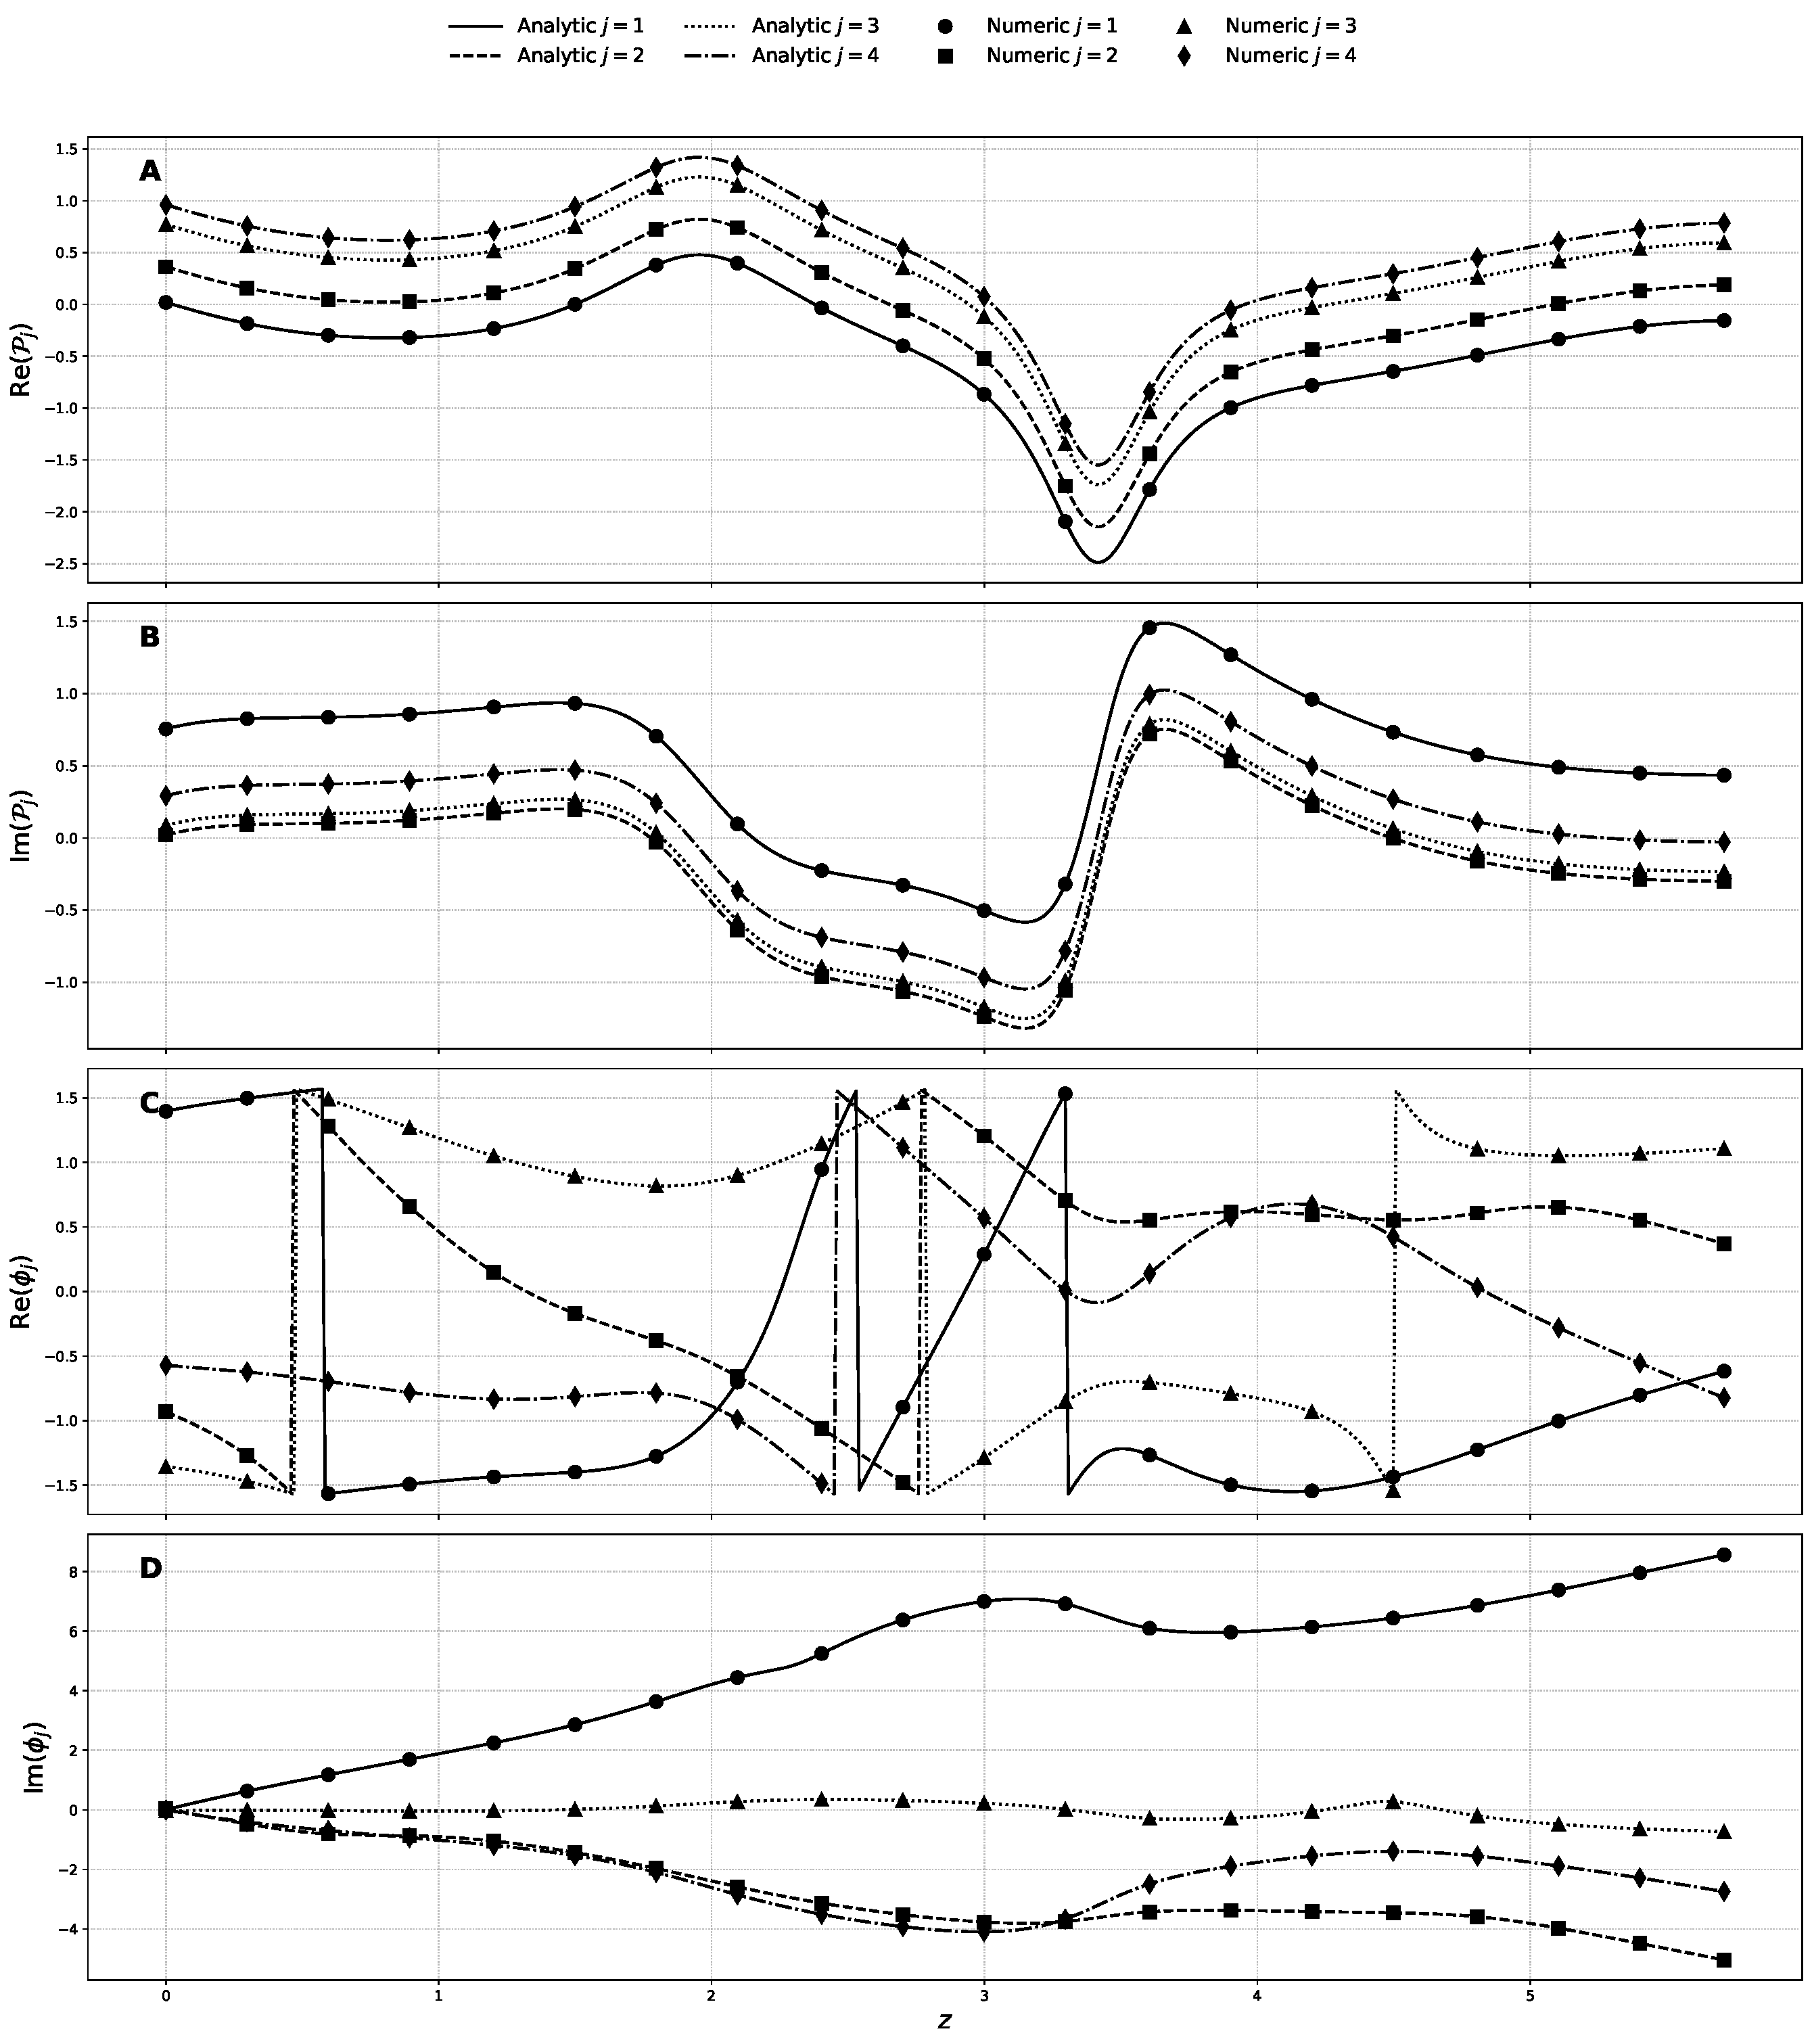
\includegraphics[width=1.0\textwidth]{plots/case1_plot_1.pdf}
\caption{\textbf{A} real and \textbf{B} imaginary parts of the complex mode power $\mathcal{P}_j=u_j v_j$, and \textbf{C} real and \textbf{D} imaginary parts of the complex phase variable $\phi_j$, using the analytic solutions in \eqref{M-eq:u-v-quartic} (dashed lines) compared against numerical integration of the abstract system \eqref{eq:uv-system} (symbols).}
\label{fig:case1-plot1}
\end{figure}

The accompanying notebook includes an additional comparison for the $d_4=0$ cubic formulas in a two-field reduction with $\Lambda_{1,j}=0$.
A separate reproducible four-mode check uses $b_2=\pm2$ with all $\Lambda_{1,j}\ne0$, checking both the zeta exponential and the linear coefficient in \eqref{eq:u-v-cubic} against the mode equations and direct integration.
The supplied audit scripts also verify the full gauge/normalisation/rescaling chain for both coupling signs and check all eight normal-form envelopes for three complex initial states; their equation residuals are below $10^{-58}$ at 60-digit working precision.

\subsection{Independent numerical projection comparison}\label{supp:subsec:projection-numeric}
The script \nolinkurl{projection_numeric_check.py} compares two independently integrated initial-value problems: the six canonical degenerate-FWM equations \eqref{cc:eq:ubar-vbar-degfwm-system} and the four gauged-coupler equations \eqref{M-cc:eq:uv-hat-system}.
No elliptic envelope is used in either integration or in their comparison.
We use the physical initial fields and asymmetric coefficients of the main paper's example, set the reciprocal gauge to the identity at $z=0$, and map the fields by \eqref{cc:eq:uv-to-jensen}.
This gives
\begin{equation}
\rho(0)=0.375,\quad (\gamma_1,\gamma_2)=(-0.475,0.475),\quad
(b_0,b_1,b_2)=(-0.875i,0.7375i,0.7i).
\end{equation}
Choose the root of the coupler quartic with largest positive imaginary part,
$\lambda_1\simeq-1.22043504+2.47690087i$.
The script refines this root and constructs the matching constants at 70-digit precision before converting to double precision for integration.
The square-root choices give $\varsigma=1$.
Fix the free lift scaling by
\begin{align}
\bar u_3(0)&=1,\qquad \bar v_3(0)=\frac{d_5}{4[\lambda_1-\rho(0)]},\notag\\
\bar u_j(0)&=\frac{\hat u_j(0)\bar v_3(0)}{\sqrt2\sqrt{\gamma_j-\lambda_1}},\qquad
\bar v_j(0)=\frac{\hat v_j(0)}{\sqrt2\sqrt{\gamma_j-\lambda_1}},\qquad j=1,2.
\end{align}
These initial data satisfy the matched weighted power differences and Hamiltonian value to better than $10^{-60}$ at the setup precision.
These complex lifted initial data realise the physical coupler initial state under the ratio projection.

Both systems are integrated separately by DOP853 over $0\le z\le8$ and sampled at 501 equally spaced points.
Only after integration do we apply \eqref{M-cc:eq:projection-hat-as-bars} to the six-component FWM solution.
The maximum absolute difference over the four projected complex components and all sample points is $6.2\times10^{-11}$ with relative/absolute tolerances $(10^{-11},10^{-13})$ and $1.6\times10^{-12}$ with tolerances $(2.5\times10^{-13},2.5\times10^{-15})$.
The latter discrepancy divided by the maximum sampled absolute target component is $1.7\times10^{-12}$; this is a scale-normalised discrepancy, not a pointwise relative error or a bound on either integration's error.
In the tighter run the maximum absolute drift of the barred Hamiltonian is $3.2\times10^{-13}$, and that of the two weighted power differences is $7.1\times10^{-13}$.
The sampled minima of $|\bar u_3|$ and $|\bar v_3|$ are approximately $0.0197$ and $1.667$, respectively, so the projection denominators remain separated from zero at the comparison points.
The script prints the complete initial states, matching constants and diagnostics in machine-readable form.

\subsection{Checks of the transformations and projection}
The accompanying coupler audit differentiates the ratio projection and verifies all four target equations together with the matched weighted power differences and Hamiltonian value.
It also checks the reconstructed original and lifted envelopes against their mode equations, including generic complex data and unequal-coefficient physical data.
The normal-form and lifted Wronskians and polynomial Lam\'e potentials are checked directly from the mode equations for both coupling signs.
These checks test the full-envelope constructions as well as the scalar power reductions.
The original symbolic and numerical notebooks are supplied unchanged as records of the manual calculations; audit scripts provide reproducible checks without rewriting their stored outputs.

\FloatBarrier

\section{FWM parameter definitions in the original coordinates}
\label{app:param-def-appendix}

This appendix provides explicit formulae for the parameters $b_l$, $c_l$, and $d_l$ that appear in the quartic polynomial \eqref{eq:drho-sqrd-3} and related expressions throughout Section~\ref{M-sec:mode-power}.
These parameters are expressed in terms of the system parameters $a_j$, $a_{j,k}$ and the conserved constants $\gamma_j$.

\begin{align}
{b}_{0} &= {a}_{0} + \sum_{j=1}^{4} {a}_{j} {\gamma}_{j} + \frac{1}{2}\sum\limits_{j,k=1}^{4} {a}_{j,k} {\gamma}_{j} {\gamma}_{k}, \notag \\
{b}_{1} &= - \sum_{j=1}^{4} {a}_{j} - \frac{1}{2}\sum\limits_{j,k=1}^{4} \left({\gamma}_{j} + {\gamma}_{k}\right) {a}_{j,k}, \notag \\
{b}_{2} &= \frac{1}{2}\sum\limits_{j,k=1}^{4} {a}_{j,k}, \notag \\
{c}_{0} &= \prod_{j=1}^{4} {\gamma}_{j}, \notag \\
{c}_{1} &= - \sum_{k=1}^{4} \prod_{\substack{j=1 \\ j \ne k}}^{4} {\gamma}_{j}, \notag \\
{c}_{2} &= \frac{3}{2} \sum_{j=1}^{4} {\gamma}_{j}^{2} - \frac{1}{4}\sum\limits_{j,k=1}^{4} \left({\gamma}_{j} - {\gamma}_{k}\right)^{2} = - \frac{1}{2}\sum_{j=1}^{4} {\gamma}_{j}^{2}, \notag \\
{d}_{0} &= {b}_{0}^{2} - 4 {c}_{0}, \notag \\
{d}_{1} &= 2 {b}_{0} {b}_{1} - 4 {c}_{1}, \notag \\
{d}_{2} &= 2 {b}_{0} {b}_{2} + {b}_{1}^{2} - 4 {c}_{2}, \notag \\
{d}_{3} &= 2 {b}_{1} {b}_{2}, \notag \\
{d}_{4} &= {b}_{2}^{2} - 4
\end{align}

% ---------- APPENDIX ------------
% --------------------------------

\section{FWM initial condition relations}
\label{app:init-conds}

This appendix gives the relationships between initial conditions for the normalised system and the constants $\gamma_j$ and $\rho(0)$ used throughout the analysis.
These relations enable determination of the constants from specified initial values of $u_j(0)$ and $v_j(0)$.

\begin{align}
\rho{\left(0 \right)} &= - \frac{1}{4}\sum_{j=1}^{4} u_j{\left(0 \right)} v_j{\left(0 \right)}, \notag \\
\left. \frac{d}{d z} \rho{\left(z \right)} \right|_{\substack{ z=0 }} &= \prod_{j=1}^{4} u_j(0) - \prod_{j=1}^{4} v_j(0), \notag \\
{\gamma}_{j} &= u_j{\left(0\right)} v_j{\left(0 \right)} + \rho{\left(0 \right)}
\end{align}


% ---------- APPENDIX ------------
% --------------------------------

\section{Parameter definitions in the bar coordinates}
\label{app:bar-coords-params}

This appendix provides the bar-coordinate parameters.
The square root $S=\sqrt{\prod_j(\gamma_j-\lambda_1)}$ is chosen as $S=\prod_j c_j/(16\lambda_1^2)$ with the same constant mode roots $c_j^2=4\lambda_1(\gamma_j-\lambda_1)$ used in Section~\ref{M-subsec:transform-domain}; hence $\varsigma=Q(\lambda_1)/(2S)$.

\begin{align}
{d}_{5} &= {d}_{1} + 2 {d}_{2} {\lambda}_{1} + 3 {d}_{3} {\lambda}_{1}^{2} + 4 {d}_{4} {\lambda}_{1}^{3}, \notag  \\
\varsigma & = \frac{1}{2} \left(b_0 + b_1 {\lambda}_{1} + b_2{\lambda}_{1}^2\right) \left(\sqrt{\prod\limits_{j=1}^4 \left(\gamma_j - \lambda_1\right)}\right)^{-1}  = \pm 1, \\
\chi &= \frac{8\left(b_0 + b_1 {\lambda}_{1} + b_2{\lambda}_{1}^2\right)}{d_5} = \frac{16\, \varsigma}{d_5}\sqrt{\prod\limits_{j=1}^4 \left(\gamma_j - \lambda_1\right)}, \notag \\
\bar{\gamma}_{j} &= \frac{{d}_{5}}{4 \left({\gamma}_{j} - {\lambda}_{1}\right)} + \frac{{b}_{1} + 2 {b}_{2} {\lambda}_{1}}{\chi} - \frac{4}{\chi^{2}}, \notag \\
{\theta}_{j} &= \frac{b_0 + b_1 {\lambda}_{1} + b_2{\lambda}_{1}^2}{2\left({\gamma}_{j} - {\lambda}_{1}\right)} + \frac{{b}_{1}}{4} + \frac{{b}_{2} {\gamma}_{j}}{2} + \frac{{b}_{2} {\lambda}_{1}}{2} - \frac{1}{\chi}, \quad \sum\limits_{j=1}^{4} \theta_j = 0, \notag \\
\bar{\kappa}_j &= 2 {\theta}_{j} + \frac{1}{\chi} - {b}_{2} {\gamma}_{j} - \zeta{\left({\mu}_{j} - z_{0}, g_2, g_3\right)}.
\end{align}

% ---------- APPENDIX ------------
% --------------------------------

\section{Scaled parameters in the tilde coordinates}
\label{app:scaled-params}
When the system in subsection \ref{M-subsec:tilde-coords} (tilde notation) is considered a transform of that in subsection \ref{M-subsec:bar-coords} (bar notation), then parameters are related via the following scaling laws:
\begin{align}
\tilde{H} &= \chi^3\bar{H}, \\
\tilde{\alpha}_j &= \frac{\varsigma}{\sqrt[4]{\varsigma}}\,\bar{\alpha}_j, \notag \\
\tilde{\gamma}_j &= \chi^2\bar{\gamma}_j, \notag \\
\tilde{g}_2 &= \chi^4 g_2, \notag \\
\tilde{g}_3 &= \chi^6 g_3, \notag \\
\xi_0 &= \frac{z_0}{\chi}, \notag \\
\tilde{\mu}_j &= \frac{\mu_j}{\chi}.
\end{align}

If the system in subsection \ref{M-subsec:tilde-coords} is considered as a standalone system irrespective of any transformation,
then the parameters can be given exclusively in the coordinate system denoted by tilde notation as follows.
Firstly, $\tilde{H}$ can be obtained from substituting $\tilde{u}_j{\left(0\right)}, \tilde{v}_j{\left(0 \right)}$ into \eqref{M-eq:H-tilde}
and $\tilde{\alpha}_j$ can be considered an integration constant fixed by initial conditions to capture any phase offset between $\tilde{u}_j, \tilde{v}_j$.
We may further use relations:
\begin{align}
\tilde{\gamma}_{j} =& \tilde{u}_j{\left(0\right)} \tilde{v}_j{\left(0 \right)} - \frac{1}{4}\sum_{j=1}^{4} \tilde{u}_j{\left(0\right)} \tilde{v}_j{\left(0\right)}, \notag \\
\tilde{g}_{2} =& \frac{\tilde{H}^{2}}{12} + \tilde{H} \left(\frac{{\tilde{e}}_{2}}{12} + \frac{16}{3}\right) + \frac{{\tilde{e}}_{2}^{2}}{48} + \frac{2 {\tilde{e}}_{2}}{3} - \frac{{\tilde{e}}_{3}}{4} + \frac{64}{3}, \notag \\
\tilde{g}_{3} =& \frac{\tilde{H}^{3}}{216} + \tilde{H}^{2} \left(\frac{{\tilde{e}}_{2}}{144} - \frac{5}{9}\right) + \tilde{H} \left(\frac{{\tilde{e}}_{2}^{2}}{288} - \frac{2 {\tilde{e}}_{2}}{9} - \frac{{\tilde{e}}_{3}}{48} - \frac{64}{9}\right) \notag \\
&+ \frac{{\tilde{e}}_{2}^{3}}{1728} - \frac{5 {\tilde{e}}_{2}^{2}}{144} - \frac{{\tilde{e}}_{2} {\tilde{e}}_{3}}{96} - \frac{8 {\tilde{e}}_{2}}{9} + \frac{{\tilde{e}}_{3}}{3} + \frac{{\tilde{e}}_{4}}{4} - \frac{512}{27}
\end{align}
where $\tilde{e}_j=\tilde{e}_j\left(\tilde{\gamma}_1, \tilde{\gamma}_2, \tilde{\gamma}_3, \tilde{\gamma}_4\right)$ is the $j^{th}$ order \emph{elementary symmetric polynomial} formed with the four $\tilde{\gamma}_j$. The points $\xi_0, \tilde{\mu}_j$ are found by inverting:
\begin{align}
\wp{\left(\xi_{0},\tilde{g}_{2},\tilde{g}_{3} \right)} &= - \frac{\tilde{H}}{12} - \frac{{\tilde{e}}_{2}}{24} - \frac{\sum_{j=1}^{4} \tilde{u}_j{\left(0\right)} \tilde{v}_j{\left(0\right)}}{4} + \frac{4}{3}, \notag \\
\wp'{\left(\xi_{0},\tilde{g}_{2},\tilde{g}_{3} \right)} &= \frac{1}{4}\left(\prod_{j=1}^{4}{\tilde{u}_j(0)} - \prod_{j=1}^{4}{\tilde{v}_j(0)}\right), \notag \\
\wp{\left({\tilde{\mu}}_{j} - \xi_{0},\tilde{g}_{2},\tilde{g}_{3} \right)} &= - \frac{\tilde{H}}{12} - \frac{{\tilde{e}}_{2}}{24} + {\tilde{\gamma}}_{j} + \frac{4}{3}, \notag \\
\wp'{\left({\tilde{\mu}}_{j} - \xi_{0},\tilde{g}_{2},\tilde{g}_{3} \right)} &= \tilde{H} + \frac{{\tilde{e}}_{2}}{4} - \frac{{\tilde{\gamma}}_{j}^{2}}{2} - 4 {\tilde{\gamma}}_{j}.
\end{align}

% ---------- APPENDIX ------------
% --------------------------------

\section{Parameters for Figure \ref{fig:case1-plot1}}
\label{app:case1-params}

\noindent
\begin{minipage}[t]{0.48\textwidth}
\centering
\captionof{table}{Initial mode values in Figure \ref{fig:case1-plot1}.}
\label{tab:case1-init}
\begin{tabular}{c c}
\hline
Variable & Initial value \\
\hline
$u_1(0)$ & $0.486-0.712i$ \\
$u_2(0)$ & $0.358-0.454i$ \\
$u_3(0)$ & $0.243-0.877i$ \\
$u_4(0)$ & $-0.918+0.413i$ \\
$v_1(0)$ & $-0.711+0.512i$ \\
$v_2(0)$ & $0.36+0.514i$ \\
$v_3(0)$ & $0.134+0.841i$ \\
$v_4(0)$ & $-0.751-0.657i$ \\
\hline
\end{tabular}
\end{minipage}
\hfill
\begin{minipage}[t]{0.48\textwidth}
\centering
\captionof{table}{Parameter values in Figure \ref{fig:case1-plot1}.}
\label{tab:case1-params}
\begin{tabular}{c c}
\hline
Parameter & Value \\
\hline
$a_1$ & $0.227$ \\
$a_2$ & $0.0474$ \\
$a_3$ & $0.17$ \\
$a_4$ & $0.874$ \\
$a_{1,1}$ & $-1.17$ \\
$a_{1,2}$ & $1.86$ \\
$a_{1,3}$ & $0.475$ \\
$a_{1,4}$ & $1.09$ \\
$a_{2,2}$ & $-1.84$ \\
$a_{2,3}$ & $-0.0376$ \\
$a_{2,4}$ & $-1.19$ \\
$a_{3,3}$ & $0.455$ \\
$a_{3,4}$ & $-0.341$ \\
$a_{4,4}$ & $-1.84$ \\
\hline
\end{tabular}
\end{minipage}

\vspace{1em}

\noindent
The coupling coefficients satisfy $a_{k,j}=a_{j,k}$.

% ---------- APPENDIX ------------
% --------------------------------

\section{Parameters for Figure \ref{M-fig:case2-plot1}}
\label{app:case2-params}
The input powers are $(1,8.5,0.4,0.01)$ W and phases are $(0.023,0.65,0.62,1.95)$ radians.
The frequency reference is $2\pi c/(1550\,\mathrm{nm})$, with offsets $(-\Omega,\Omega,-3\Omega,3\Omega)$ and $\Omega=2\pi\times100$ GHz.
The propagation constants are $\beta_j=\tfrac12\beta^{(2)}(\omega_j-\omega_{\rm ref})^2$ with their common mean subtracted, where $\beta^{(2)}=-30\,\mathrm{ps}^2/\mathrm{km}$.
These choices preserve frequency conservation and give nonzero phase mismatch.

\begin{table}[H]\centering
\caption{Initial field amplitudes for Figure~\ref{M-fig:case2-plot1}; $|A_j|^2$ is in watts.}
\label{tab:case2-init}
\begin{tabular}{cc}\hline Variable & Initial value \\ \hline
$A_1(0)$ & $0.99973551+0.02299797i$ \\
$A_2(0)$ & $2.32096317+1.76440641i$ \\
$A_3(0)$ & $0.51474193+0.36747890i$ \\
$A_4(0)$ & $-0.03701808+0.09289597i$ \\
\hline\end{tabular}\end{table}
\begin{table}[H]\centering
\caption{Parameters for Figure~\ref{M-fig:case2-plot1}; entries are rounded.}
\label{tab:case2-physical}
\begin{tabular}{cc}\hline Parameter & Value \\ \hline
$c$ & $299792458$ [m/s] \\
$n_2$ & $2.6\times10^{-20}$ [$\mathrm m^2/\mathrm W$] \\
$A_{\rm eff}$ & $10\times10^{-12}$ [$\mathrm m^2$] \\
$\beta^{(2)}$ (GVD) & $-3\times10^{-26}$ [$\mathrm s^2/\mathrm m$] \\
$\omega_1$ & $1.21463076\times10^{15}$ [rad/s] \\
$\omega_2$ & $1.21588739\times10^{15}$ [rad/s] \\
$\omega_3$ & $1.21337412\times10^{15}$ [rad/s] \\
$\omega_4$ & $1.21714403\times10^{15}$ [rad/s] \\
$\beta_1$ & $0.0236870506$ [1/m] \\
$\beta_2$ & $0.0236870506$ [1/m] \\
$\beta_3$ & $-0.0236870506$ [1/m] \\
$\beta_4$ & $-0.0236870506$ [1/m] \\
\hline\end{tabular}\end{table}
The common overlap approximation is $f_{j,k}=f_{1,2,3,4}=1/A_{\rm eff}=1.0\times10^{11}\,\mathrm m^{-2}$ for all indices.
The notebook supplies full-precision inputs.

\section{Coherent-coupler parameter definitions}
\label{cc:app:param-def-appendix}

This appendix provides explicit formulae for the parameters $b_l$, $c_l$, and $d_l$ that appear in the quartic polynomial \eqref{cc:eq:drho-sqrd-3} and related expressions throughout Section~\ref{cc:sec:mode-power}.
These parameters are expressed in terms of the system parameters $a_j$, $a_{j,k}$ and the conserved constants $\gamma_j$.

\begin{align}
N &= 2,\\
{b}_{0} &= {a}_{0} + \sum_{j=1}^{N} {a}_{j} {\gamma}_{j} + \frac{1}{2}\sum\limits_{j,k=1}^{N} {a}_{j,k} {\gamma}_{j} {\gamma}_{k}, \notag \\
{b}_{1} &= - \sum_{j=1}^{N} {a}_{j} - \frac{1}{2}\sum\limits_{j,k=1}^{N} \left({\gamma}_{j} + {\gamma}_{k}\right) {a}_{j,k}, \notag \\
{b}_{2} &= \frac{1}{N}\sum\limits_{j,k=1}^{N} {a}_{j,k}, \notag \\
{c}_{0} &= \prod_{j=1}^{N} {\gamma}_{j}, \notag \\
{d}_{0} &= {b}_{0}^{2} - 4 {c}_{0}, \notag \\
{d}_{1} &= 2 {b}_{0} {b}_{1}, \notag \\
{d}_{2} &= 2 {b}_{0} {b}_{2} + {b}_{1}^{2} - 4, \notag \\
{d}_{3} &= 2 {b}_{1} {b}_{2}, \notag \\
{d}_{4} &= {b}_{2}^{2}
\end{align}

% ---------- APPENDIX ------------
% --------------------------------

\section{Coherent-coupler initial condition relations}
\label{cc:app:init-conds}

This appendix gives the relationships between initial conditions for the physical system and the constants $\gamma_j$ and $\rho(0)$ used throughout the analysis.
These relations enable determination of the constants from specified initial values of $u_j(0)$ and $v_j(0)$.

\begin{align}
N &= 2, \notag \\
\rho{\left(0 \right)} &= - \frac{1}{N}\sum_{j=1}^{N} u_j{\left(0 \right)} v_j{\left(0 \right)}, \notag \\
\left. \frac{d}{d z} \rho{\left(z \right)} \right|_{\substack{ z=0 }} &= \prod_{j=1}^{N} u_j(0) - \prod_{j=1}^{N} v_j(0), \notag \\
{\gamma}_{j} &= u_j{\left(0\right)} v_j{\left(0 \right)} + \rho{\left(0 \right)}
\end{align}


% ---------- APPENDIX ------------
% --------------------------------

\FloatBarrier
\begingroup
\emergencystretch=2em
\printbibliography
\endgroup
\end{document}
